%%%%%%%%%%%%%%%%%%%%%%%%%%%%%%%%%%%%%%%%%%%%%%%%%%%%%%%%%%%%%%%%%%%%%%%%%%%%%%%%
%2345678901234567890123456789012345678901234567890123456789012345678901234567890
%        1         2         3         4         5         6         7         8

\documentclass[letterpaper, 10 pt, conference]{ieeeconf}  % Comment this line out if you need a4paper

%\documentclass[a4paper, 10pt, conference]{ieeeconf}      % Use this line for a4 paper

\IEEEoverridecommandlockouts                              % This command is only needed if 
                                                          % you want to use the \thanks command

\overrideIEEEmargins                                      % Needed to meet printer requirements.

\usepackage{amsmath,amssymb,url,times,subfigure,graphicx,theorem}
\usepackage{graphicx,subfigure,hyperref}
\usepackage{color,comment}
\usepackage{csquotes}
%\usepackage{refcheck}

\usepackage{epic,eepic}

%\usepackage[]{algorithm2e}
\usepackage[linesnumbered,ruled,vlined]{algorithm2e} 

\graphicspath{{../../Fig/}}

\newcommand{\norm}[1]{\ensuremath{\left\| #1 \right\|}}
\newcommand{\abs}[1]{\ensuremath{\left| #1 \right|}}
\newcommand{\bracket}[1]{\ensuremath{\left[ #1 \right]}}
\newcommand{\braces}[1]{\ensuremath{\left\{ #1 \right\}}}
\newcommand{\parenth}[1]{\ensuremath{\left( #1 \right)}}
\newcommand{\ip}[1]{\ensuremath{\langle #1 \rangle}}
\newcommand{\refeqn}[1]{(\ref{eqn:#1})}
\newcommand{\reffig}[1]{Fig. \ref{fig:#1}}
\newcommand{\tr}[1]{\mbox{tr}\ensuremath{\negthickspace\bracket{#1}}}
\newcommand{\trs}[1]{\mbox{tr}\ensuremath{\!\bracket{#1}}}
\newcommand{\deriv}[2]{\ensuremath{\frac{\partial #1}{\partial #2}}}
\newcommand{\G}{\ensuremath{\mathsf{G}}}
\newcommand{\SO}{\ensuremath{\mathsf{SO(3)}}}
\newcommand{\T}{\ensuremath{\mathsf{T}}}
\renewcommand{\L}{\ensuremath{\mathsf{L}}}
\newcommand{\so}{\ensuremath{\mathfrak{so}(3)}}
\newcommand{\SE}{\ensuremath{\mathsf{SE(3)}}}
\newcommand{\se}{\ensuremath{\mathfrak{se}(3)}}
\renewcommand{\Re}{\ensuremath{\mathbb{R}}}
\newcommand{\Sph}{\ensuremath{\mathsf{S}}}
\newcommand{\aSE}[2]{\ensuremath{\begin{bmatrix}#1&#2\\0&1\end{bmatrix}}}
\newcommand{\ase}[2]{\ensuremath{\begin{bmatrix}#1&#2\\0&0\end{bmatrix}}}
\newcommand{\D}{\ensuremath{\mathbf{D}}}
\renewcommand{\d}{\ensuremath{\mathbf{d}}}
\newcommand{\pair}[1]{\ensuremath{\left\langle #1 \right\rangle}}
\newcommand{\met}[1]{\ensuremath{\langle\!\langle #1 \rangle\!\rangle}}
\newcommand{\Ad}{\ensuremath{\mathrm{Ad}}}
\newcommand{\ad}{\ensuremath{\mathrm{ad}}}
\newcommand{\g}{\ensuremath{\mathfrak{g}}}
\newcommand{\argmin}{\operatornamewithlimits{argmin}}
\newcommand{\argmax}{\operatornamewithlimits{argmax}}

\title{\LARGE \bf
Bidding-Based Autonomous Exploration of Cooperative Robots Building a 3D Probabilistic Occupancy Grid Map}

\author{Evan Kaufman and Taeyoung Lee%
\thanks{Evan Kaufman, Taeyoung Lee, Mechanical and Aerospace Engineering, George Washington University, Washington DC 20052 {\tt \{evankaufman,tylee\}@gwu.edu}}
\thanks{This research has been supported by the U.S. Naval Research Laboratory Base Program Work Unit ``Intelligent Microflyer'' and in part by NSF under the grants CMMI-1243000, CMMI-1335008, and CNS-1337722.}
}


\newtheorem{definition}{Definition}
\newtheorem{lem}{Lemma}
\newtheorem{prop}{Proposition}
\newtheorem{cor}{Corollary}
\newtheorem{remark}{Remark}


\begin{document}



\maketitle
\thispagestyle{empty}
\pagestyle{empty}


%%%%%%%%%%%%%%%%%%%%%%%%%%%%%%%%%%%%%%%%%%%%%%%%%%%%%%%%%%%%%%%%%%%%%%%%%%%%%%%%
\begin{abstract}

This paper presents a bidding-based cooperative robotic exploration strategy to generate accurate occupancy grid maps with multiple vehicles. Using recent developments in 3D occupancy grid mapping and autonomous exploration, we propose an auction-based framework to build maps from various vantage points. A central executive reviews individual robot bids to maximize map information gain, and these bids are updated to prevent robots from capturing the same grid cells or colliding, which is further optimized with a receding horizon framework. Furthermore, considering a multi-agent system capable of large environmental coverage, several computational enhancements are presented to improve the scalability of the mapping and exploration algorithms. This multi-vehicle exploration approach is demonstrated with a numerical simulation where three robots simultaneously explore a large building floor plan cooperatively.

\end{abstract}


%%%%%%%%%%%%%%%%%%%%%%%%%%%%%%%%%%%%%%%%%%%%%%%%%%%%%%%%%%%%%%%%%%%%%%%%%%%%%%%%
\section{Introduction}


Robotic mapping is the process of generating maps representing the environment surrounding robots.
Mapping serves an important role in tasks such as search-and-rescue, surveillance, and robotic cleaning.
Several grid-based map representations have been studied, e.g.,~\cite{WolSuk05,MeyBeiBur12,TanThoWolBus14}, because they provide abundant occupancy knowledge about the environment and are computationally tractable. 

Most grid-based mapping representations are designed for 2D, while others are extended to capture a full 3D environment. In particular, occupancy probabilities have been assigned to a uniform 3D grid in~\cite{Andert09,PirRutBisSch11}. Another highly-popular variation of occupancy grid mapping is the Octomap representation~\cite{WurHorBenStaBur10,HorWurBenStaBur13}, which has added features such as extending the mapping limits and changing cell sizes. Most recently,~\cite{KauLeeAiMos16,KauTakAiLee17} proposed a systematic method to build an accurate probabilistic map using depth sensor stochastic properties directly, which is extended to 3D in~\cite{KauTakAiLee18}.

Next consider how the motions of cooperating robots impact the knowledge of a 3D map, known as autonomous exploration. 
A common approach is known as frontier-based exploration, proposed for 2D environments in~\cite{Yam97,Yam98} and extended to 3D  using the Octomap representation in~\cite{ZhuDinLinWu15,SenWan16,KleDor13}, and similarly using a visibility metric in~\cite{SawKriSri09}. This approach moves robots toward the boarder between certain and uncertain spaces, though these systematic actions are not based on any consideration of the future probabilistic map uncertainty.

Alternatively, there have been exploration techniques that are based on a quantitative measure of uncertainty known as Shannon's entropy~\cite{StaGriBur05}, and it is used to acquire expected map information gain in~\cite{KauAiLee16,KauTakAiLee17} in 2D. Here, the robot selects actions to learn the largest amount about the map using expected entropy \emph{change}. This concept is extended to 3D environments in~\cite{KauTakAiLee18}, where important properties of the 3D occupancy grid are projected onto a 2D map to eliminate computational costs. However, this approach governs robotic motion of just a single vehicle. 

In this paper, we propose to expand the uncertainty-based exploration technique for multiple robots mapping cooperatively. However, optimizing map coverage simultaneously from multiple vehicles becomes very complicated and computationally intractable. Instead, an auction-based approach addresses the computational restrictions effectively. Bidding-based approaches were introduced with~\cite{SimApfBurFoxMooThrYou00,DiaSte00}, and extended to several other robotic problems~\cite{GerMaj02,ZloSteDiaTha02,SarBal05,ChoBruHow09} exploring decentralization and task allocation with varying robot capabilities. In~\cite{SimApfBurFoxMooThrYou00}, a central executive assigns tasks to robots for maximizing overall utility of the group. This is accomplished by minimizing a coverage overlap among the members. Robots submit bids based on expected coverage of uncertain spaces and travel distance. The robot winning the auction is awarded the task, and the remaining bids are discounted to prevent robots from covering the same area, thereby coordinating the mapping efforts.

% probabilistic map uncertainty to generate bids

Here, we propose an alternative multi-vehicle coordinated exploration approach that uses a central executive, focussed on map information gain maximization. Instead of estimating coverage overlap among robots, the proposed approach predicts how robotic actions are expected to improve map information gain cooperatively in a probabilistic fashion. A series of auctions determines where robots should travel. During each auction, robots submit bids based on how their sensors are expected to improve the quality of the occupancy grid map. Between auctions, bids are modified to reflect the impact of other robot members on the map. Because this approach is directly based on cooperative improvement of map information, considering coverage overlap among the robots becomes unnecessary. This multi-vehicle exploration optimization is further augmented with travel time considerations and collision avoidance among robots. In short, the proposed multi-vehicle exploration scheme employs a bidding framework that maximizes map information while considering multiple vehicles cooperating together.




%Expected changes in Shannon's entropy of the probabilistic map in conjunction with robot travel distances provide sufficient information for the bids from several candidate poses. Then, a novel bid discounting method provides a means for multi-vehicle coordination. This discounting method is composed of two parts: first, the expected information gains within the neighborhood of winning bids are updated based on how the winning bid is expected to change the map, thereby avoiding coverage overlapping among robots. Second, bids are further discounted with a cost associated with Euclidean distance to avoid collisions between exploring robots. In short, the robot locations and expected entropy of the occupancy grid map are considered together to avoid coverage overlaps or collisions.

Furthermore, this bidding-based exploration approach is integrated with a receding horizon framework to optimize map information and collision-avoidance in a dynamic environment. The receding horizon framework serves to update the exploration strategy with a possibly-changing occupancy grid map, which directly impacts the viability of pose candidates. Additionally, a receding horizon provides an optimal feedback policy that can handle dynamic obstacles, such as collision-avoidance with cooperative robots.

Finally, we present a numerical simulation of three quadrotors mapping and exploring a floor plan of a building. Since the environment is particularly large, this motivates several algorithm modifications to promote operational scalability, where communication among the various processes is focussed on map changes and multithreading is applied where necessary, among other computational enhancements.

The paper is organized as follows. The mapping and exploration problems are formulated in Section \ref{sec:ProbDef}. The method for auctioning exploration bids with receding horizons is presented in Section \ref{sec:BiddingExploration}. A mapping and exploration simulation with a scalable solution is shown in Section \ref{sec:NumericalSim}, followed by conclusions.


\section{Problem Formulation}
\label{sec:ProbDef}

This sections summarizes the key equations providing the exact solutions to occupancy grid mapping and expected entropy change proposed in~\cite{KauLeeAiMos16,KauTakAiLee17,KauTakAiLee18,KauAiLee16}.

\subsection{Probabilistic Occupancy Grid Mapping}
\label{subsec:POGM}
Let map $m$ be an occupancy grid map decomposed into $n_m$ evenly-spaced cubic grid cells with fixed edge length $\alpha$. The $i$-th grid cell is assigned to a static binary random variable $\mathbf{m}_i$ for $i\in\braces{1,2,\ldots,n_m}$, that is defined as $\mathbf{m}_i=1$ when occupied, and $\mathbf{m}_i=0$ when free. The location and size of each grid cell is assumed known, where a smaller cell size better represents a space, but increases computation and memory. Therefore, a map $m$ is defined by $\{\mathbf{m}_1,\ldots, \mathbf{m}_{n_m}\}$ ($2^{n_m}$ possible maps).

Another random variable is defined as $\bar{\mathbf{m}}_i=1-\mathbf{m}_i$ for convenience, which is the event that the $i$-th cell is free, i.e., $P(\bar{\mathbf{m}}_i)=1-P(\mathbf{m}_i)$. The random variables composing $m$ are assumed mutually independent, 
\begin{align}
P(m)=P(\mathbf{m}_1,\mathbf{m}_2,\ldots,\mathbf{m}_{n_m})=\prod_{i=1}^{n_m}P(\mathbf{m}_i).
\end{align}

% {R ? R3�3 | RT R = I, det R = 1}
Consider a range sensor that provides scans of the surrounding environment in order to identify the closest occupied space. Let the measurement scan at the $t$-th time step be $Z_t$, where $z\in Z_t$ is a single measurement ray. Let the $t$-th pose be denoted by $X_t=\braces{x_t,R_t}$ with location $x_t\in\Re^3$ and attitude $R_t\in\SO=\braces{R\in\Re^{3\times3}|R^\T R=I,\det{R}=1}$, where $X_t$ is assumed to be known, i.e., perfect localization is considered. Given the sensor probabilistic properties $p(z|X_t,m)$, commonly referred to as the \emph{forward sensor model}, the goal is finding the \emph{inverse sensor model}, $P(m|z,X_{1:t},Z_{1:t-1})$. To obtain this probability for all cells,~\cite{KauLeeAiMos16,KauTakAiLee17} introduced a reduced map $r\subset m$ composed of $n_r$ cells along $z$, where cells are indexed by increasing distance from $x_t$, and $\mathbf{r}_{k+}$ refers to the event that the $k$-th cell of map $r$ is the closest occupied space. Then, the inverse sensor model for the $k$-th cell is
\begin{align}
\label{eqn:RayISMAnswer}
P(\mathbf{r}_{k}|z,X_{1:t},Z_{1:t-1})&=\eta\tilde P(\mathbf{r}_{k}|z,X_{1:t},Z_{1:t-1}),
\end{align}
where $\eta$ is the normalizer,
\begin{align}
\label{eqn:allEta}
\eta
&=
\bigg[\sum_{i=1}^{n_{r}+1}\bigg\{\prod_{j=0}^{i-1}\bar{\mathbf{P}}_j^-\bigg\} p(z|\mathbf{r}_{i+},X_t)\mathbf{P}_i^-\bigg]^{-1},
\end{align}
such that the probability summation of the entire space is $1$, and the unnormalized probability of the inverse sensor model is defined as
\begin{align}
\label{eqn:Unnormalized}
\tilde P(\mathbf{r}_{k}|z,X_{1:t},&Z_{1:t-1})\nonumber\\
&=\mathbf{P}_k^-
\bigg[\sum_{i=1}^{k-1}\bigg\{\prod_{j=0}^{i-1}\bar{\mathbf{P}}_j^-\bigg\}p(z|\mathbf{r}_{i+},X_t)\mathbf{P}_k^-\bigg]\nonumber\\
&\quad + \bigg\{\prod_{j=0}^{k-1}\bar{\mathbf{P}}_j^-\bigg\}p(z|\mathbf{r}_{k+},X_t)\mathbf{P}_k^-,
\end{align}
where a priori probability is $\mathbf{P}_k^-=P(\mathbf{r}_{k}|X_{1:t-1},Z_{1:t-1})$, its complement is $\bar{\mathbf{P}}_k^-=1-\mathbf{P}_k^-$, $P(\bar{\mathbf{r}}_{0}|X_{1:t-1},Z_{1:t-1})=P(\mathbf{r}_{n_r+1}|X_{1:t-1},Z_{1:t-1})=1$ for convenience, and $p(z|\mathbf{r}_{(n_r+1)+},X_t)$ represents the forward sensor model of a maximum sensor reading.The proofs of \refeqn{RayISMAnswer}--\refeqn{allEta} are given in~\cite{KauLeeAiMos16}. Since the terms of \refeqn{Unnormalized} are easily obtained and several are used repeatedly to obtain \refeqn{allEta}, the computational cost of \refeqn{RayISMAnswer} is trivial and can be applied in real-time. This process is repeated for all measurements composing scan $Z_t$.

\subsection{Predictive Entropy-Based Autonomous Exploration}


Since occupancy grid mapping provides a probabilistic representation of surrounding space, this mapping scheme holds probabilistic information about the uncertainty of the map. Shannon's entropy is commonly used as a measure of uncertainty, such as in~\cite{StaGriBur05}. Given the probabilities of each grid cell of map $m$, Shannon's entropy of an individual cell and the entire map are defined as
\begin{align}
\label{eqn:ShannonsEntropyCell}
H(P(\mathbf{m}_i))&=-P(\mathbf{m}_i)\log{P(\mathbf{m}_i})-P(\bar{\mathbf{m}}_i)\log{P(\bar{\mathbf{m}}_i}),
\\
\label{eqn:ShannonsEntropyMap}
H(P(m))&=\sum_{i=1}^{n_m}H(P(\mathbf{m}_i)),
\end{align}
respectively.
The entropy of the $i$-th grid cell is maximized when $P(\mathbf{m}_i)=0.5$ (greatest uncertainty) and minimized as $P(\mathbf{m}_i)$ approaches $0$ or $1$ (smallest uncertainty). %; thus Shannon's entropy is a measure of uncertainty.

Let an unvisited candidate future pose and its measurement scan be $X_c=\braces{x_c,R_c}$ and $Z_c$, respectively, such that $c\in\mathcal C$ where $\mathcal C=\braces{1,2,...,n_c}$ is the set of all $n_c$ candidates. Since the robot has not visited $X_c$, any change to the probabilistic map must be predicted. Much like the probabilistic mapping, this is achieved ray-by-ray~\cite{KauAiLee16,KauTakAiLee17}. Since all grid cell probabilities are conditioned on the history of poses $X_{1:t}$ and measurement scans $Z_{1:t}$, these are removed from the remaining equations for simplicity. For candidate ray $z_c$, the expected entropy is
\begin{align}
\label{eqn:DiscExpEntropyRay}
&\text{E}[H(P(m|x_c,z_{c}))]=\sum_{k=1}^{n_{r}+1}\bigg\{H(P(m|x_c,z_{c,k}))P(z_{c,k}|x_c)\bigg\},
\end{align}
where subscript $k$ refers to the event that the candidate \emph{measurement} captures the $k$-th cell along the ray, i.e., $z_{c,k}$ is the distance from $x_c$ to the $k$-th grid cell. The first term of the summation of \refeqn{DiscExpEntropyRay}, namely $H(P(m|x_c,z_{c,k}))$, is obtained with the inverse sensor model \refeqn{RayISMAnswer}--\refeqn{allEta} and entropy definitions \refeqn{ShannonsEntropyCell}, \refeqn{ShannonsEntropyMap}. The second term is found using \refeqn{allEta} with
\begin{align}
\label{eqn:ProbMeas}
P(z_{c,k}|x_c)&=\frac{p(z_{c,k}|x_c)}{\sum_{i=1}^{n_{r}+1}p(z_{c,i}|x_c)}=\frac{\eta_{c,k}^{-1}}{\sum_{i=1}^{n_{r}+1}\eta_{c,i}^{-1}},
\end{align}
where $\eta_{c,k}$ refers to the normalizer calculated with $z_{c,k}$.
Then, the expected information gain for candidate pose $X_c$ is the negative entropy change,
\begin{align}
%\label{eqn:objectiveFunOptimized}
%X_c^*&=\argmax_{X_c}{\ \mathcal I(X_c)},
%\\
\label{eqn:expectedInfoGainRay}
\mathcal I(X_c)&=H(P(m|X_{1:t},Z_{1:t}))-\text{E}\left[H(P(m|X_c,Z_c))\right],
\end{align}
where \refeqn{DiscExpEntropyRay} is used repeatedly for several sample rays that compose scan $Z_c$ as shown in~\cite{KauAiLee16}. Assuming the sample rays are spaced sufficiently apart, each ray tends to intersect a different set of grid cells, so these rays composing $Z_c$ are considered independently.

\section{Bidding-Based Autonomous Exploration}
\label{sec:BiddingExploration}

Here, we formulate a cooperative exploration problem with multiple robots using sequential auctions. The first auction is based on the expected information gain presented in the prior section, scaled by travel distance. Once the winner of the first auction is determined, the map for bidding is updated based on the expected measurements of the first robot. The second auction for the remaining robots is determined by the information gain from the revised map that is further scaled by the travel distance and a penalty for collision-avoidance. This process is repeated until all robots are assigned tasks. Then, the robots traverse toward their optimal poses while the bidding process repeats using a receding horizon framework.

%The expected information gain of each robot can be obtained from the computation framework presented in the prior section. As such, we consider the cost of travel and multi-vehicle coordination in this section.

%We assume that all robots mapping the environment use the same set of depth sensors to update the grid cells. Then, \refeqn{expectedInfoGainRay} is valid for all robots, and the total candidate information gains outlined in~\cite{KauAiLee16} need only be calculated once during a set of auctions. The only aspect differentiating robot bids is travel distance. The completed bids, and discounting for multi-vehicle coordination, are described next.

\subsection{Objective Function for the First Auction}

Instead of considering the full 3D map during entropy calculations, which yields a more complicated and computationally expensive information gain expectation, we project the 3D map onto a simpler 2D map, namely $m_\text{2D}$, located at the robot altitude according to~\cite{KauTakAiLee18}. The main idea is that several 3D cells in each dimension serve to update a single 2D projected cell probability, accounting for collision and entropy. This approach conservatively and efficiently captures small occupied spaces around the robot height. However, this approach is not suitable for capturing floors and ceilings or exploring complex 3D environments such multi-level buildings or complex terrain. Since these features are not considered for exploration here, we apply the map projection technique to the multi-vehicle autonomous exploration problem.



%. Consider a candidate pose $X_c$. Even though $\mathcal I(X_c)$ is fixed because the set $\mathcal I=\braces{\mathcal I_1,\mathcal I_2,\ldots,\mathcal I_{n_c}}$ is fixed, the travel time for each robot can differ greatly. This motivates a unified approach to differentiate bids for the same candidate pose from different robots.

%The expected information gain $\mathcal I(X_c)$ from \refeqn{expectedInfoGainRay} is identical for all robots. Therefore the same set $\mathcal I=\braces{\mathcal I_1,\mathcal I_2,\ldots,\mathcal I_{n_c}}$ can be applied for all robots. However

%; in some cases, certain robots, or even all robots, cannot reach $X_c$

Next, we describe how travel time is integrated into exploration. Considering that distances from current robot poses to candidate poses may differ greatly, accounting for these varying travel times properly is essential for exploration time efficiency. Travel distances are computed using Dijkstra's search to provide collision-free waypoints for each robot. There are two steps: first, generate a cost map from the robot location to each location on the 2D projected map. This provides the collision-free distances to all reachable locations on the map, which is different than the Euclidean distance in general. Second, the waypoints from a candidate pose to the current robot pose are easily obtained along the cost map using steepest descent. 

%    if x(k) < d
%        f(k) = 0.5*fMax*(1-cos(pi*x(k)/d));
%    else
%        f(k) = fDiff*exp(-1e-2*(x(k)-d)^2)+fFar;
%    end


%Dijkstra's search demonstrates that the distances from each robot to $X_c$ are different in general, so travel times to $X_c$ vary. This motivates a unified approach to account for travel time, which promotes local travel and discourages robots from traversing across the map when possible.

Here, we define a bump function to account for varying travel distances from Dijkstra's search. Let the distance along the collision-free path from the $k$-th robot pose, namely $X_k$, to the $c$-th candidate pose, namely $X_c$, be denoted $d(X_k,X_c,m_\text{2D})\geq0$, which is taken from the cost map belonging to $X_k$. A continuous bump function is defined to account for traveling costs, and is composed of two parts.  

The first part of the bump function corresponds to short trajectories. Consider $d_\text{opt}$, the time-optimal distance that a robot may travel at full speed during the time between exploration updates. Here, we consider the case when $d(X_k,X_c,m_\text{2D})\leq d_\text{opt}$, i.e., the robot can completely traverse this distance during the allotted travel time. If $d(X_k,X_c,m_\text{2D})\ll d_\text{opt}$, then the robot is not moving at its full potential. This can be wasteful, because the robot tends to capture larger regions while moving. Therefore, it is desirable for $d(X_k,X_c,m_\text{2D})\rightarrow d_\text{opt}$, which corresponds to maximizing map coverage without time cost. The first part of the bump function is sinusoidal and is optimized at $d_\text{opt}$ to maximize robotic movement as
\begin{align}
\mathcal B_1(d)=\frac12\mathcal B_\text{max}\left(1-\cos{\frac{d\pi}{d_\text{opt}}}\right),
\end{align}
where $\mathcal B_\text{max}>0$ is the maximum value when $d(X_k,X_c,m_\text{2D})=d_\text{opt}$.

The second part of the bump function is defined over the domain where $d(X_k,X_c,m_\text{2D})>d_\text{opt}$ to minimize time required for $X_k$ to arrive at $X_c$, prioritizing local movements rather than traversing across the environment. This choice is beneficial to generating accurate local maps before exploring new regions. The second half is defined to be nonzero everywhere and strictly decreasing as 
\begin{align}
\mathcal B_2(d)=(\mathcal B_\text{max}-\mathcal B_\text{far})\exp\braces{-\beta(d_\text{opt}-d)^2}+\mathcal B_\text{far},
\end{align}
where $\mathcal B_\text{max}>\mathcal B_\text{far}>0$ guarantees $\mathcal B_2>0$ such that $\mathcal B_2\rightarrow \mathcal B_\text{far}$ as $d(X_k,X_c,m_\text{2D})\rightarrow\infty$ and $\beta>0$ assigns the rate of functional decrease relative to $\mathcal B_\text{max}$ and $\mathcal B_\text{far}$. Then, the complete bump function is defined as
\begin{align}
\label{eqn:bumpFun}
\mathcal B(d)=
\begin{cases}
    \mathcal B_1(d),		& \text{if }d\leq d_\text{opt},\\
    \mathcal B_2(d),         & \text{otherwise},
\end{cases}
\end{align}
which is illustrated in Fig. \ref{fig:nonzeroBumpFun}. % In short, the bump function prioritizes short movements to capture the local environment over long traversals for exploration time efficiency.

	\begin{figure}
		\centerline{
			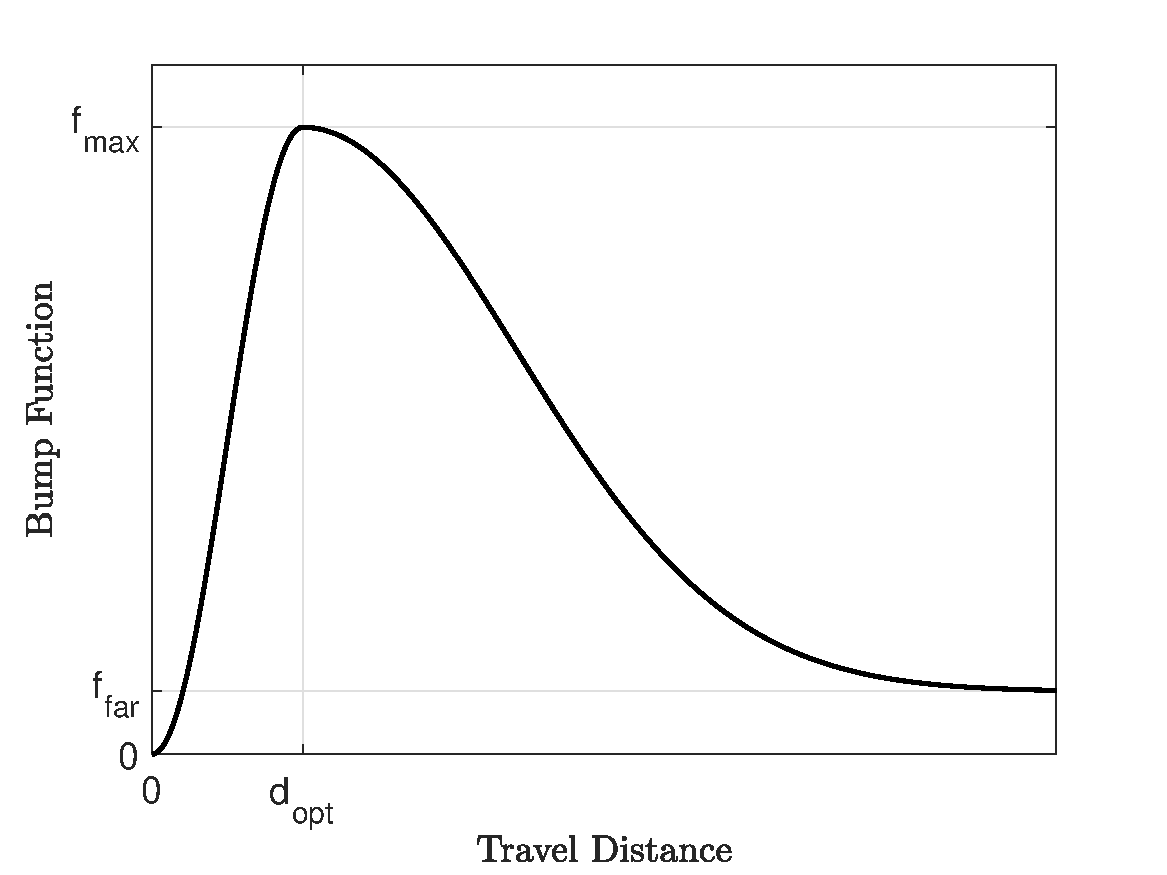
\includegraphics[width=0.9\columnwidth]{NonZeroBump.pdf}
		}
		\caption{Bump Function to Optimize Robot Exploration Time}
		\label{fig:nonzeroBumpFun}
	\end{figure}
	
Then, using the information gain from \refeqn{expectedInfoGainRay} and considering the impact from travel distance from \refeqn{bumpFun}, the objective function for a single agent with respect to $X_{c}$ is
\begin{align}
\label{eqn:CandidateBidSingle}
\text{Obj}_\text{single}(X_k,X_c,m_\text{2D})&=\mathcal B(d(X_k,X_c,m_\text{2D}))\mathcal I(X_{c},m_\text{2D}).
%X_{k,c}^*&=\argmax_{X_c}{\ \mathcal B_{k,c}\mathcal I(X_c)},
\end{align}
Then, the optimal pose selection for the $k$-th agent is
\begin{align}
\label{eqn:OptPoseSingle}
X^*_{k}=\argmax_{X_c}\text{Obj}_\text{single}(X_k,X_c,m_\text{2D}).
\end{align}
Therefore, the bump function from \refeqn{bumpFun} prioritizes robotic movement within the local surrounding space before the robot moves across the map to distant regions, while still considering faraway pose candidates.

The first auction includes bids from all robots, and proceeds as follows. Let the set of all $n_R$ robots be denoted $\mathcal R=\braces{R_1,R_2,\dots,R_{n_R}}$ such that the $k$-th robot, namely $R_k$, bids $\text{Obj}_\text{single}(X^*_k,X_c,m_\text{2D})$ from \refeqn{CandidateBidSingle} and \refeqn{OptPoseSingle}. This is repeated for all $k$ such that $R_k\in\mathcal R$. The robot with the largest bid wins the first auction at index $k^*$, and is assigned to travel to $X^*_{k^*}$. Then, the remaining robots must account for $R_{k^*}$ in subsequent auctions, described next.

\subsection{Subsequent Auctions}

The robots unable to win the first auction are updated to reflect the expected impact of $R_{k^*}$. This robot is expected to modify the probabilistic occupancy grid map, which may significantly change the expected information gains and collision properties of candidate poses nearby $X^*_{k^*}$. The process of auctioning and modifying bids is repeated, removing the winning robot from consideration after each auction, until no robots remain. Between auctions, updating the map with expected measurements from auction-winning robots discourages the remaining robots from entering the same regions and capturing the same cells. As such, there is no need to consider the coverage overlap explicitly: it is avoided in a systematic way as increased coverage overlap would reduce the overall information gain.

% Furthermore, an additional term serves to avoid collisions between robots.

%When agents submit their first candidate bid, namely $\text{Obj}_\text{single}(X^*_k,X_c,m_\text{2D})$ from \refeqn{CandidateBidSingle} and \refeqn{OptPoseSingle}, this serves to maximize the expected information gain of the map while accounting for distance. However, this bid alone disregards the impact of other robots. Hence, using bids generated this way repeatedly would lead to uncoordinated robot efforts.

More specifically, we coordinate robotic efforts by modifying bids to prevent robots from updating the same grid cells and to avoid collisions among robots. The goal is to find the winning bids $\mathcal X^*=\braces{X^*_{1},X^*_{2},\dots,X^*_{n_R}}$ corresponding to each robot from $\mathcal R$. During the auctioning process, let $\mathcal W\subset\mathcal R$ be the set of robots that have already won auctions by producing the largest objective function bid. After the first auction described above, $\mathcal W=\braces{R_{k^*}}$; after all auctions are complete, $\mathcal W=\mathcal R$. Between auctions, the candidate poses are modified for information gain and collision-avoidance, coordinating the multi-vehicle exploration.

% The main idea is that accounting for the expected change in the occupancy grid map from an auction-winning robot provides a multi-vehicle exploration policy that avoids excessive coverage of the same grid cells.

The first step between auctions is to modify the expected map information gain for efficient map coverage.  Once a robot wins a bid, the measurement ray expected values serve to update a temporary copy of $m_\text{2D}$, namely $m_\text{2D,copy}$, and those candidates located in a local neighborhood (twice the radius of a maximum sensor reading) of the winning candidate from the prior auction are recalculated, thereby coordinating total map information gain with auction-winning robots. Using the same local map notation from \refeqn{allEta} and \refeqn{Unnormalized} along a measurement ray, the expected measurement value is
\begin{align}
\label{eqn:ExpectedMeasRay}
\text{E}[z]=\sum_{k=1}^{n_{r}}\bigg\{\prod_{j=0}^{k-1}\bar{\mathbf{P}}_j^-\bigg\}\mathbf{P}_k^-z_k,
\end{align}
where $z_k$ denotes the distance from the robot sensor to the $k$-th cell along the measurement ray. Then $\text{E}[z]$ is substituted into \refeqn{RayISMAnswer}--\refeqn{Unnormalized} to modify $m_\text{2D,copy}$, and expected map information gains are recomputed with \refeqn{ProbMeas} and \refeqn{expectedInfoGainRay}, while the bump function \refeqn{bumpFun} remains the same.

The second step focusses on collision-avoidance between robots based on their proximity. Let $\rho_\text{max}>0$ be a fixed maximum radius to consider collision-avoidance and $\rho_{i,c}\geq0$ be the Euclidean distance from the $i$-th already-assigned pose $X^*_i$ to the $c$-th candidate pose $X_c$, i.e.,
\begin{align}
\rho_{i,c}&=\norm{x^*_i-x_c},
\end{align}
where $x^*_i$ and $x_c$ are the pose locations of $X^*_i$ and $X_c$, respectively. Then the collision-avoidance factor for the $k$-th robot such that $R_k\notin\mathcal W$ is,
\begin{align}
\label{eqn:CollisionAvoidanceAmongRobots}
\mathbf C(X_c)&=
\begin{cases}
    \prod_{i|\mathcal{R}_i\in\mathcal W} \left(\frac{\rho_{i,c}}{\rho_\text{max}}\right)^2,		& \text{if }\rho_{i,c}<\rho_\text{max},\\
    1,              				& \text{otherwise},
\end{cases}
\end{align}
where this product serves to decrease the value of bids for candidate poses in close proximity with already-assigned poses to avoid collisions between robots. The multi-vehicle objective function for the $k$-th robot accounting for collision-avoidance is
\begin{align}
\label{eqn:CandidateBidMulti}
\text{Obj}_\text{multi}&(X_k,X_c,m_\text{2D,copy})
\nonumber\\&=\mathbf C(X_c)\mathcal B(d(X_k,X_c,m_\text{2D}))\mathcal I(X_{c},m_\text{2D,copy}),
\end{align}
where its optimal pose during this auction is
\begin{align}
\label{eqn:OptPoseMulti}
X^*_{k}=\argmax_{X_c}\text{Obj}_\text{multi}&(X_k,X_c,m_\text{2D,copy}),
\end{align}
where $\text{Obj}_\text{multi}(X^*_k,X_c,m_\text{2D,copy})$ is the bid for the $k$-th robot.
Optimal pose selection and bidding is repeated for all robots not belonging to $\mathcal W$. The largest bid among these wins the auction and is tasked with moving to the associated pose candidate, and then this robot is included with $\mathcal W$ to avoid further consideration. Completing $n_R$ auctions produces $\mathcal X^*$.


The proposed approach uses auctions and bid modifications based on total map information gain and collision-avoidance, promoting exploration of different spaces without explicit consideration of coverage overlaps. The pseudocode for the bidding process is shown with Algorithm \ref{alg:bidding}, and a high level diagram of the entire process is illustrated with \ref{fig:MultiVehicleAutonomousExplorationDiagram}.

\begin{algorithm}
	Function: $Bidding(\mathcal X_r,\mathcal I(X_c)\forall c\in\mathcal C,\rho_\text{max})$\;
	Initialize $k=0$, $\mathcal W=0_{n_R\times1}$, $B=0_{n_R\times1}$\;
	Update candidate expected information gains using \refeqn{DiscExpEntropyRay}\;
	\For{$i=n_R,n_R-1,\ldots,1$}{
		\For{$j=1,2,\ldots,n_R$}{
			\If{$\mathcal W(j)==0$}{
				\If{$i==n_R$}{
					Maximize bid \refeqn{CandidateBidSingle} for $X^*_{j}$ from \refeqn{OptPoseSingle}\;
				}
				\Else{
					Update $\mathcal I(X_c)$ close to $\mathcal X^*(k)$\;
					\For{$c=1,2,\ldots,n_c$}{
						Find Euclidean distance $\rho_{k,c}$\;
					Get $\mathbf C(X_c)$ with \refeqn{CollisionAvoidanceAmongRobots}\;
					}
					Maximize bid \refeqn{CandidateBidMulti} for $X^*_{j}$ from \refeqn{OptPoseMulti}\;
				}
				Insert the $j$-th maximum bid into $B(j)$\;
			}
		}
		$k$: index maximizing $B$ with corresponding $X^*_{k}$\;
		$\mathcal X^*(k)=X^*_{k}$\;
		$\mathcal W(k)=1$\;
		$B(k)=0$\;
	}

	Return $\mathcal X^*$\;
\caption{Robot Task Bidding}
\label{alg:bidding}
\end{algorithm}



	\begin{figure}
		\centerline{
			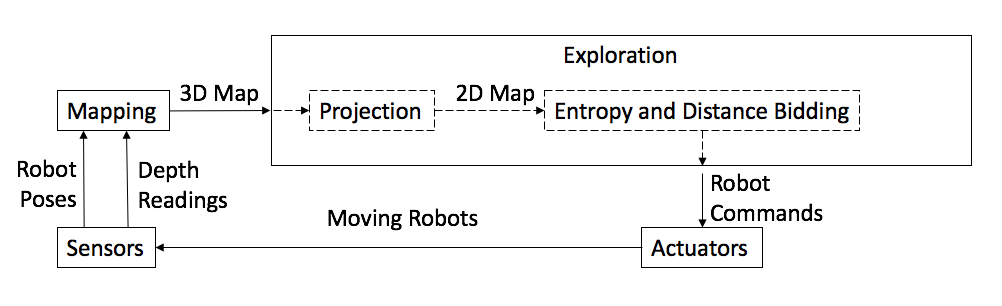
\includegraphics[width=0.9\columnwidth]{MultiVehicleAutonomousExplorationDiagram.png}
		}
		\caption{Multi-Vehicle Autonomous Exploration Diagram}
		\label{fig:MultiVehicleAutonomousExplorationDiagram}
	\end{figure}
	


\subsection{Receding Horizon Framework}
This algorithm is further aided by following a receding horizon framework for improved information gain maximizations and collision-avoidance with dynamic obstacles such as other robots. A receding horizon simply repeats the autonomous exploration steps as quickly as possible, frequently before a robot reaches its desired pose. Since exploration optimizations can only occur during exploration updates, a receding horizon maximizes the rate at which these updates occur. These updates require time for computation, over which the robot can move $d_\text{opt}$, used to optimize the robot travel distances with \refeqn{bumpFun}. Hence, the receding horizon framework serves to repeat optimizations as quickly as possible with maximal robotic movement while exploring a changing occupancy grid.

Furthermore, a receding horizon framework enhances autonomous exploration in two other ways. First, the occupancy grid map is constantly updated while a robot traverses a trajectory, so the expected information gains change as well. Since the bids depend on the occupancy grid, $\mathcal X^*$ is updated accordingly. This prevents robots from completing trajectories that have become unnecessary as new terrain becomes captured. Second, the receding horizon prevents robots from colliding with each other when they become too close together (e.g., crossing paths, traversing a tight passage). The cost map for each robot is updated, and the location of other robots are considered as collision-prone space. Hence, the robot trajectories become better separated due to rapid updates of the cost maps with the receding horizon. 


\section{Numerical Results}
\label{sec:NumericalSim}

\subsection{Software Structure}

The algorithms for mapping, exploration, and visualization are designed for the Robot Operating System (ROS). This framework allows the node that computes 3D mapping probabilities to easily transfer these to an exploration node and a visualization node. The exploration node is separated into three threads running in parallel. The first thread constantly updates the 2D projected map according to~\cite{KauTakAiLee18}. The second thread computes the information gains, runs auctions, and generates trajectories. The third thread broadcasts a message for visualizing the 2D projected map. This structure is chosen because the 2D map cannot afford to miss messages, and the last two may produce time bottlenecks and are independent of each other. The final node is for 3D map visualization, and it creates a message to the ROS visualization package, Rviz, to produce 3D cells with varying opacities corresponding to cell occupancy probabilities.

The multi-vehicle exploration problem is typically applied to large environments, so several scalability precautions are taken to avoid large communications and computations. Most importantly, only the map \emph{changes} are communicated from the mapping node to the exploration and visualization nodes using a custom message type. This change drastically decreases the time needed to generate or interpret the message. This is accomplished by finding a rectangular prism of the minimum and maximum limits of cells that may have changed during a particular measurement scan update. Publishing and subscribing to map changes provides an efficient means to transfer mapping information, independent of map size.

Another computational improvement key to autonomous exploration success is that only important and changing map information gains are updated. The expected information gain for a single candidate is updated ray-by-ray, as demonstrated in~\cite{KauTakAiLee17,KauTakAiLee18}. For every measurement ray, only the top $n_p$ cells with the largest detection probabilities are considered. Since \refeqn{ProbMeas} is embedded in \refeqn{DiscExpEntropyRay}, the computational complexity for a ray with $n_{r}$ cells is $\mathcal O(n_{r}^2)$. Reducing the considered cells to $n_p$ limits the computation to $\mathcal O(n_{p}^2)$ where $n_{p}\ll n_r$ in general. Furthermore, finding these $n_p$ cells is computationally inexpensive; using a selection algorithm of the $n_{r}$ cells and a sorting algorithm of the $n_{p}$ cells, the computational complexity is amortized to $\mathcal O(n_r+n_p\log(n_p))$. This entropy updating scheme scales well to varying sensor ranges and cell sizes. Furthermore, the information gains of poses far from any robot trajectory need not be updated between receding horizons.


\subsection{Parameters and Resulting Maps}
The 3D mapping and exploration algorithms for three robots are simulated with several parameters, which are the same as those presented in~\cite{KauTakAiLee18} except the map limits are extended to $-55.0$m to $55.0$m in the x- and y-directions, and $0.0$m to $1.5$m in the z-direction, producing a total of 45,255,504 grid cells with edge length $0.075$m (dimensioned $1468\times1468\times21$). For the bump function, $\mathcal B_\text{max}=1$, $\mathcal B_\text{far}=0.1$, and $\beta=0.01$ are chosen. For bidding $\rho_\text{max}=3.0$m is chosen.



In the simulation, three quadrotors explore the simulated environment of The George Washington University's (GWU) Science and Engineering Hall (SEH) for $10$ minutes while taking measurements. Each quadrotor is given an Asus Xtion depth sensor and Hokuyo LIDAR, where the sensor properties for the Asus Xtion are used with exploration expectations because they provide the vast majority of measurements. The building floor plan and Gazebo simulated environment are shown in Fig. \ref{fig:SEHEnvironment}. The 3D occupancy grid maps are shown in Fig. \ref{fig:sim3DMap}, and the corresponding 2D projected maps for exploration are shown in Fig. \ref{fig:sim2Dmaps} using the ROS visualization package Rviz. The full video of both maps is available at https://youtu.be/OMn2c453oik.


	\begin{figure}
		\centerline{
			\subfigure[Floor Plan]{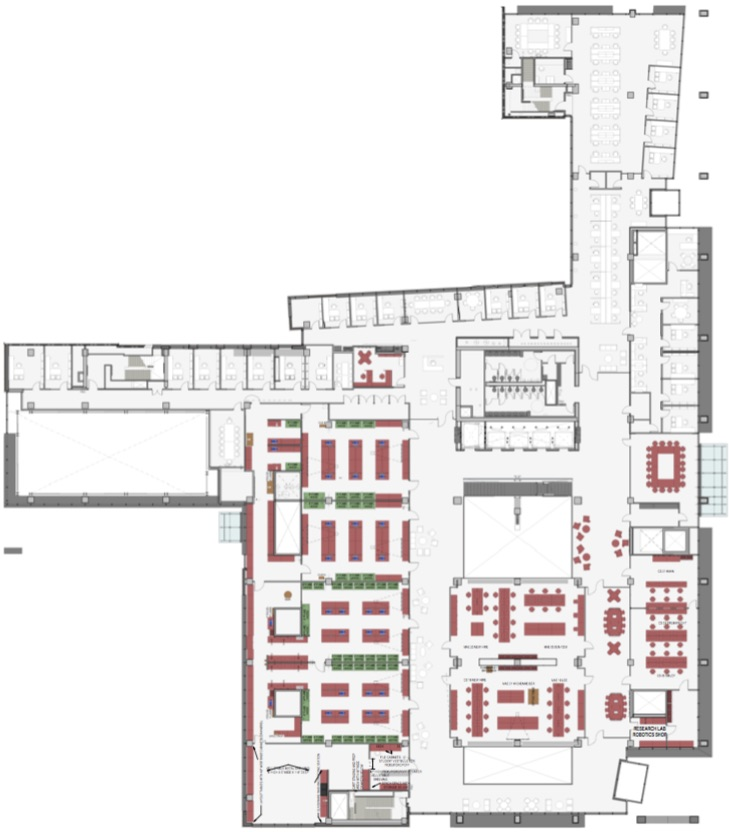
\includegraphics[height=0.5\columnwidth]{SEH_cropped.jpeg}}
			\hspace*{0.025\columnwidth}
			\subfigure[Gazebo Environment]{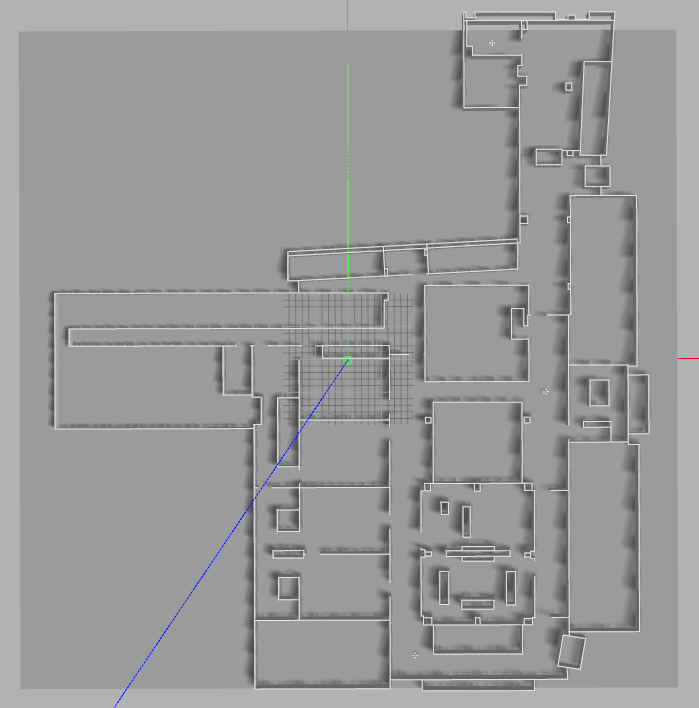
\includegraphics[height=0.5\columnwidth]{gazeboSEH.png}}
		}
		\caption{Simulated Environment of SEH}
			\label{fig:SEHEnvironment}
	\end{figure}

	\begin{figure}
	% trim={<left> <lower> <right> <upper>}
		\centerline{
			\subfigure[$0$ min]{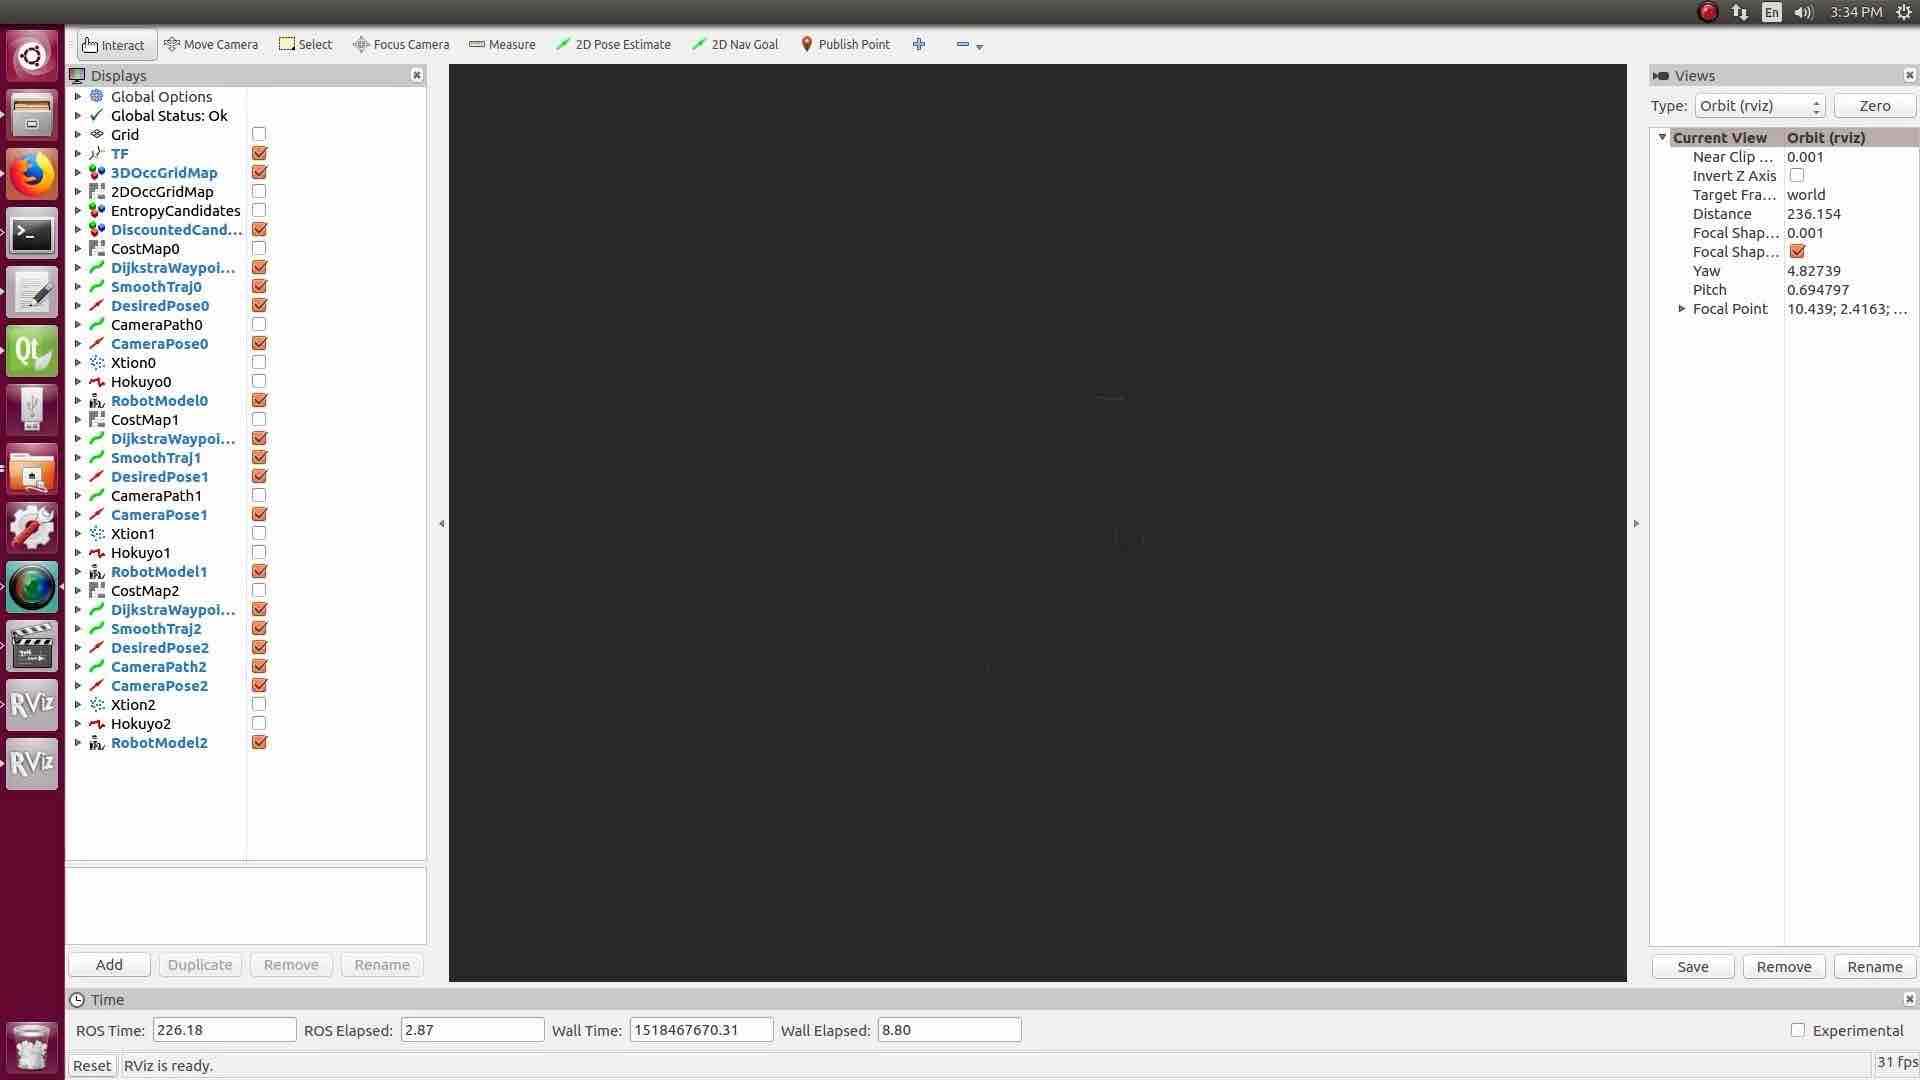
\includegraphics[trim={26cm 10cm 24cm 10cm}, clip, height=0.45\columnwidth]{multi_discount_raw_3D_0min_ss.jpg}}
			\hspace*{0.025\columnwidth}
			\subfigure[$1$ min]{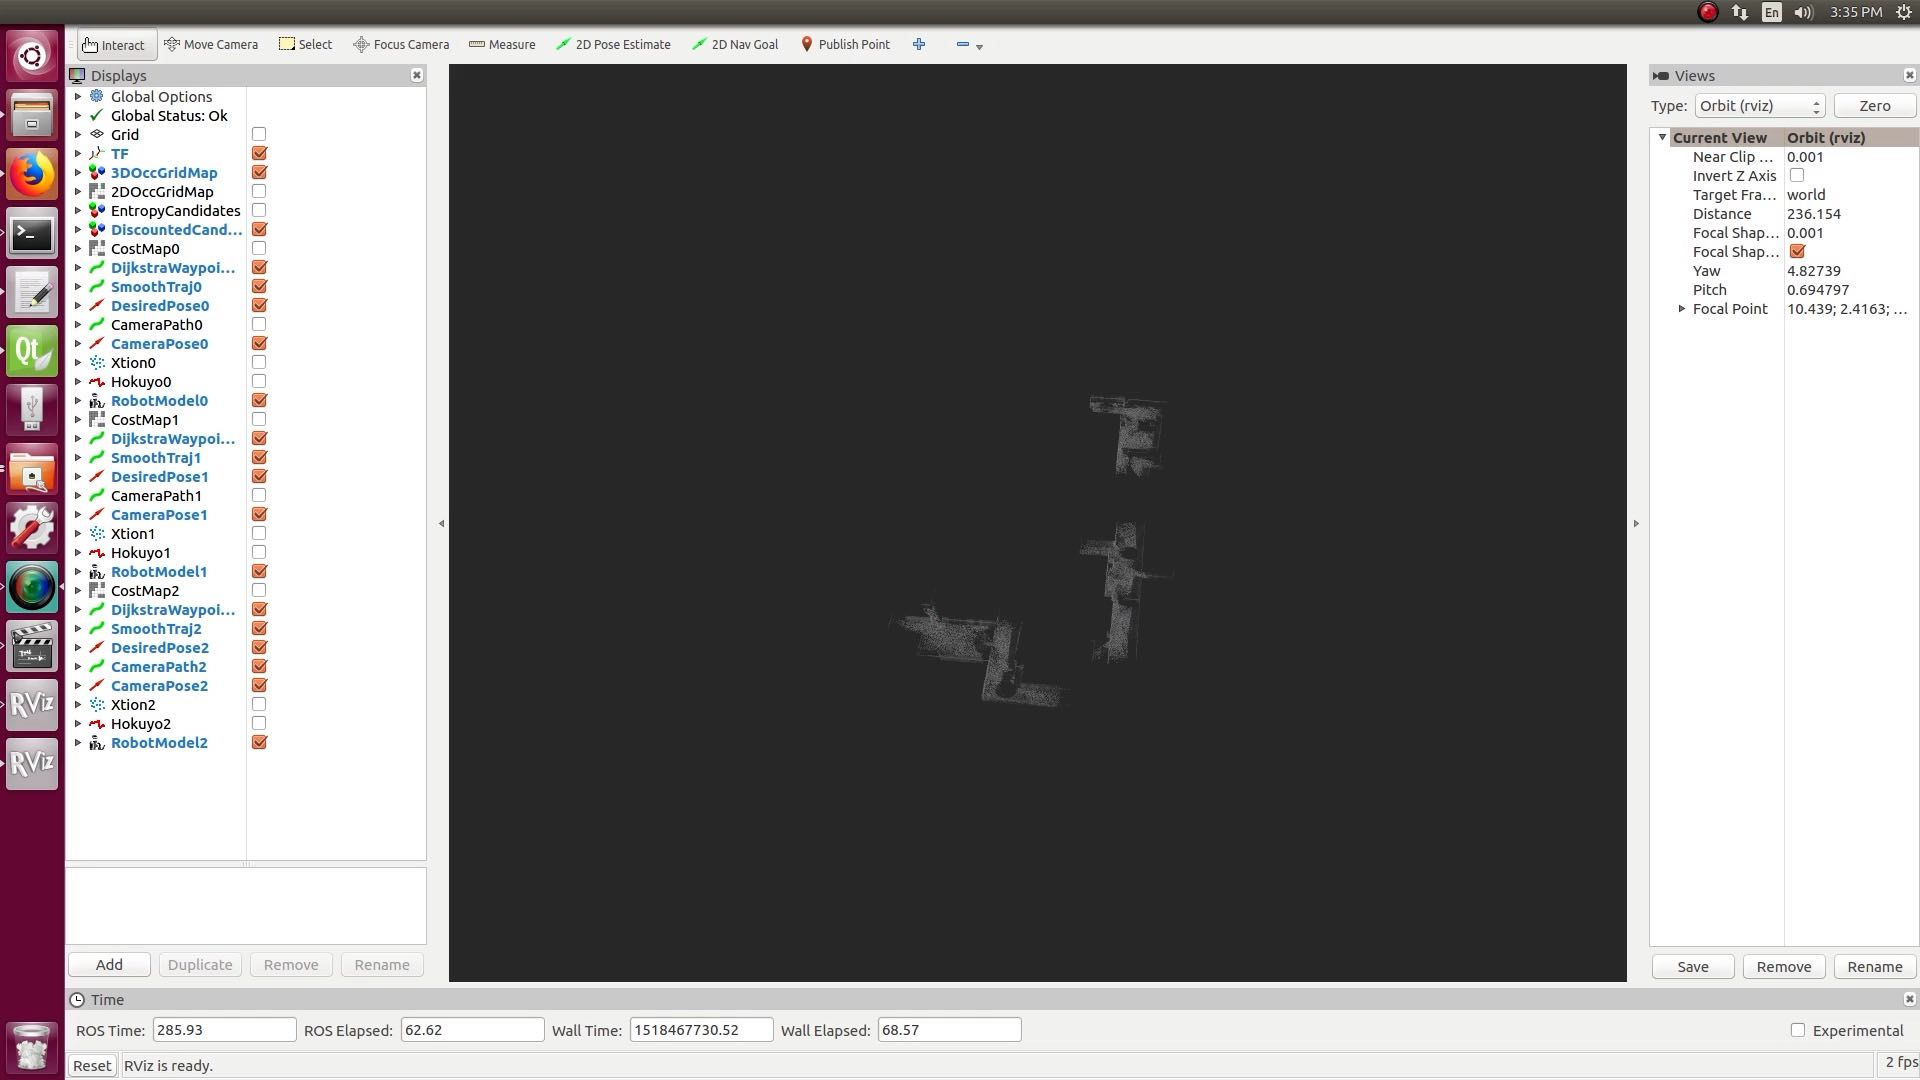
\includegraphics[trim={26cm 10cm 24cm 10cm}, clip, height=0.45\columnwidth]{multi_discount_raw_3D_1min_ss.jpg}}
		}
		\vspace*{0.025\columnwidth}
		\centerline{
			\subfigure[$2$ min]{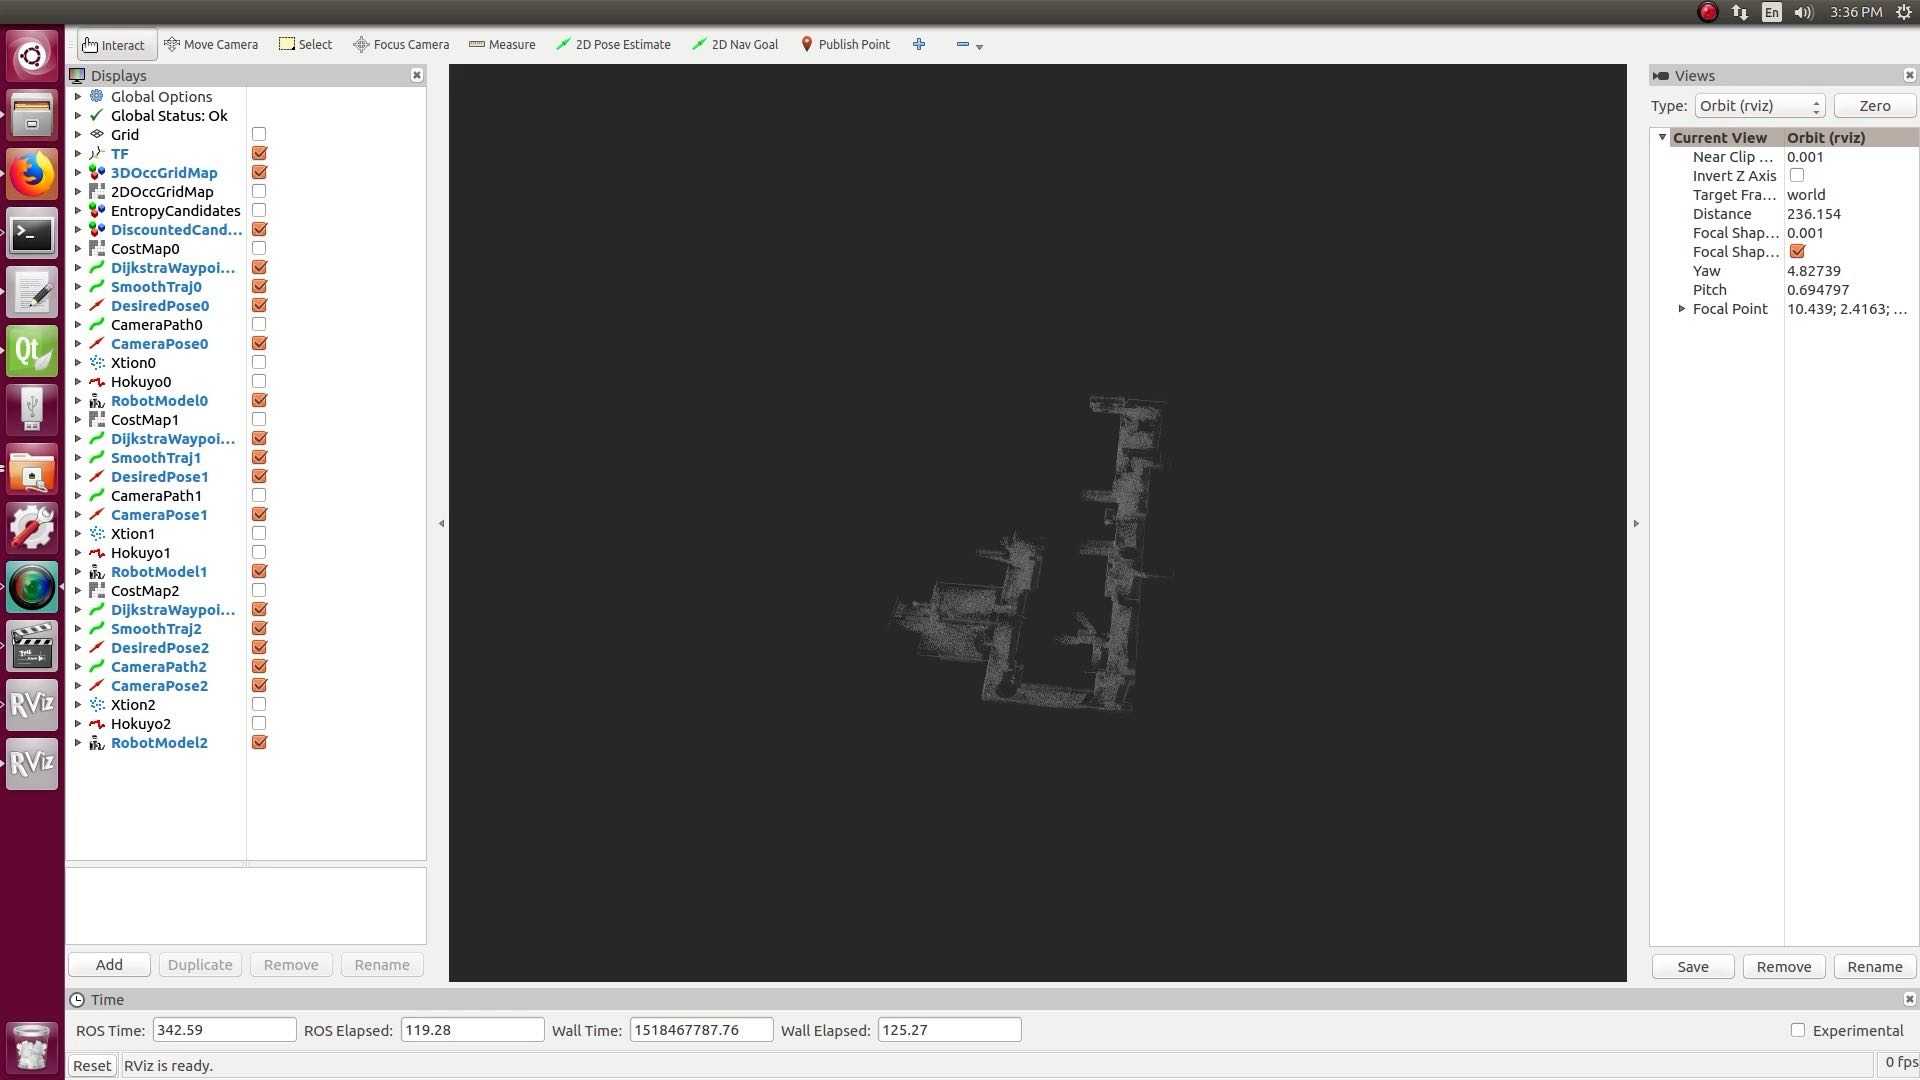
\includegraphics[trim={26cm 10cm 24cm 10cm}, clip, height=0.45\columnwidth]{multi_discount_raw_3D_2min_ss.jpg}}
			\hspace*{0.025\columnwidth}
			\subfigure[$3$ min]{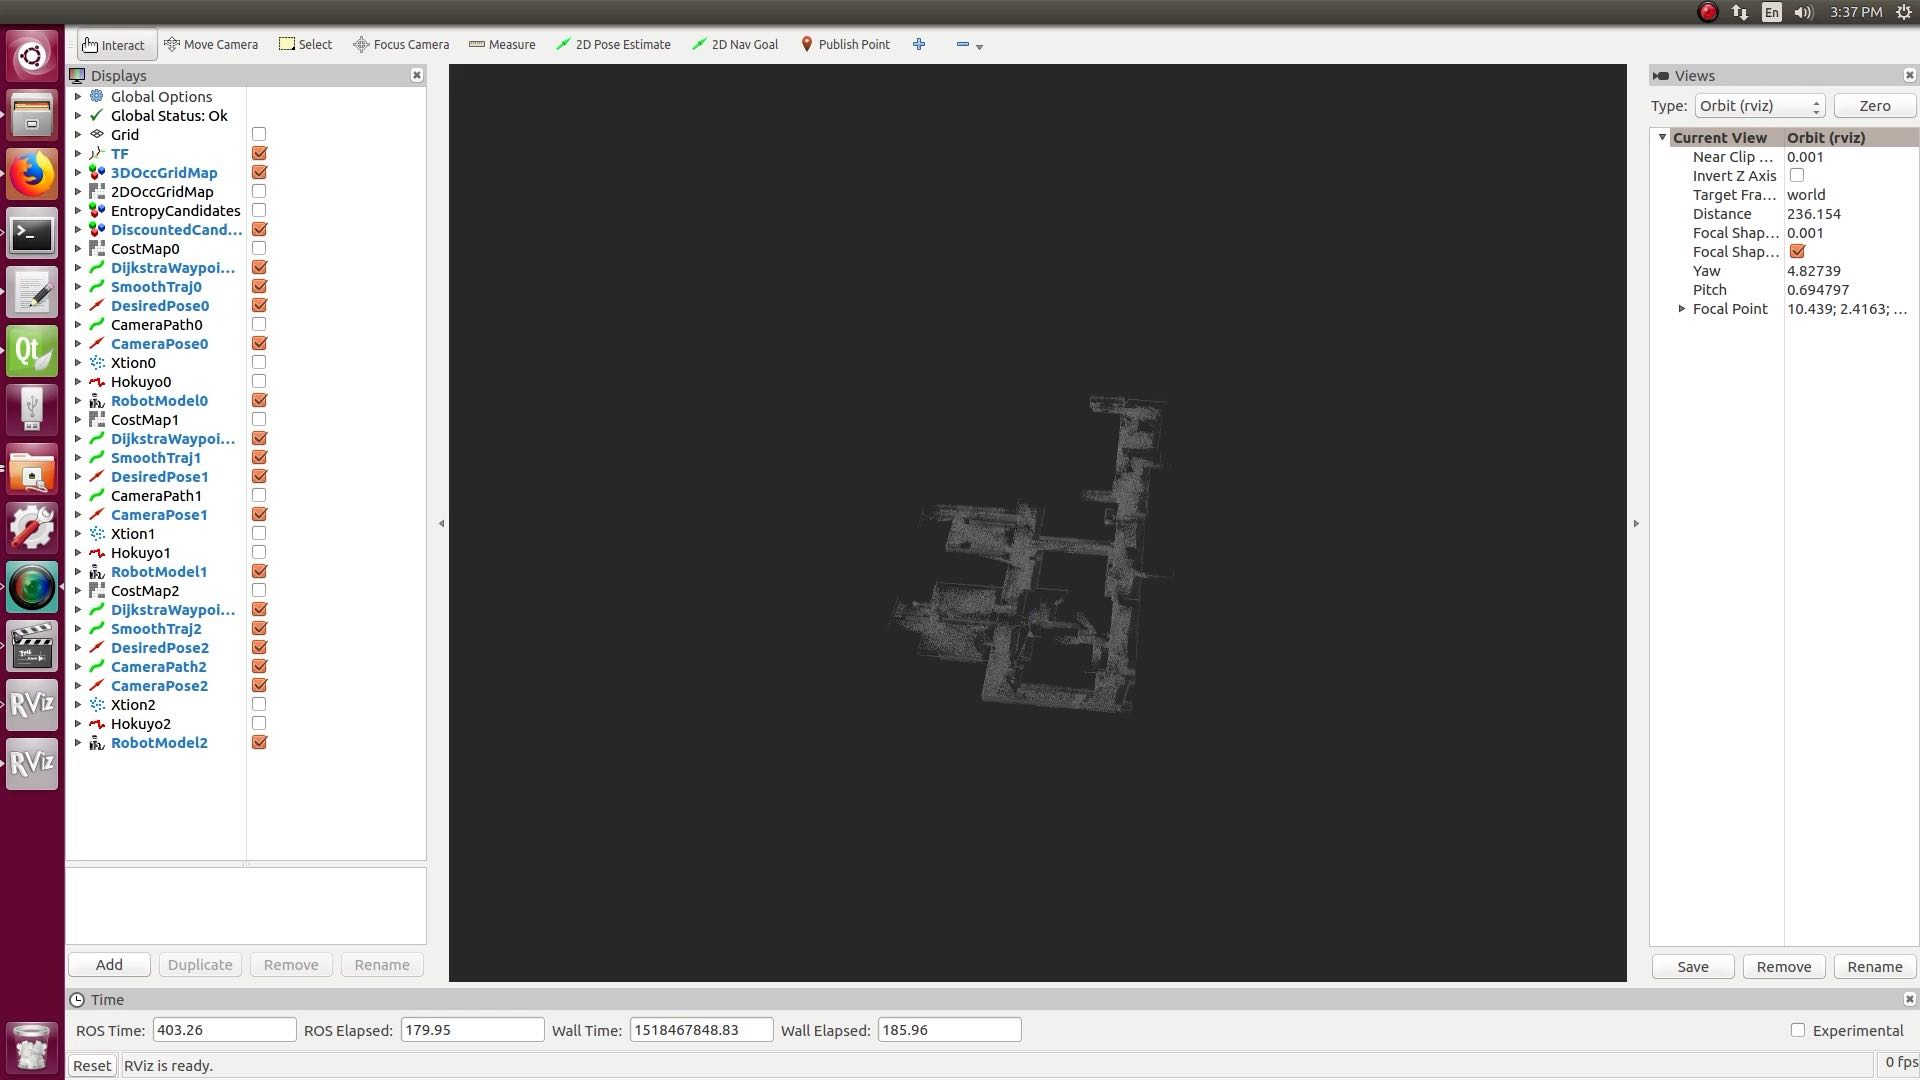
\includegraphics[trim={26cm 10cm 24cm 10cm}, clip, height=0.45\columnwidth]{multi_discount_raw_3D_3min_ss.jpg}}
		}
		\vspace*{0.025\columnwidth}
		\centerline{
			\subfigure[$4$ min]{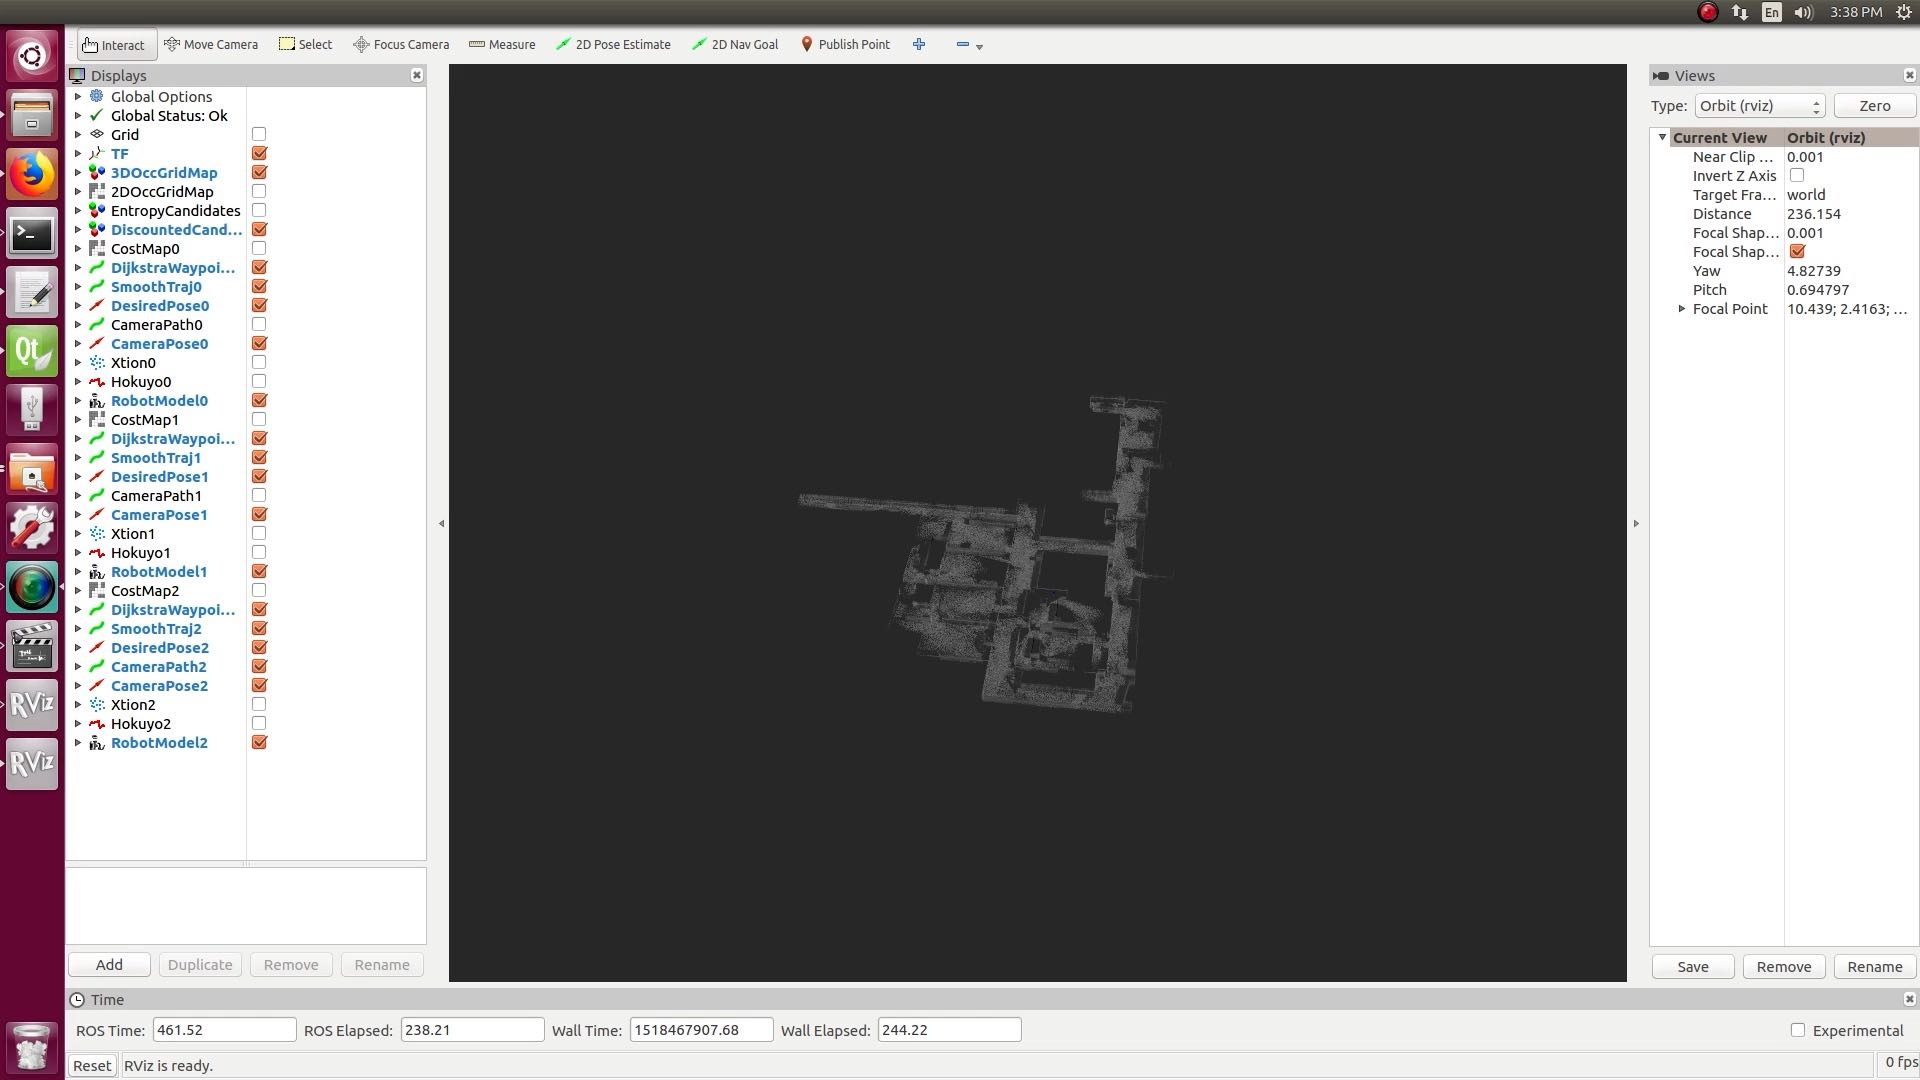
\includegraphics[trim={26cm 10cm 24cm 10cm}, clip, height=0.45\columnwidth]{multi_discount_raw_3D_4min_ss.jpg}}
			\hspace*{0.025\columnwidth}
			\subfigure[$5$ min]{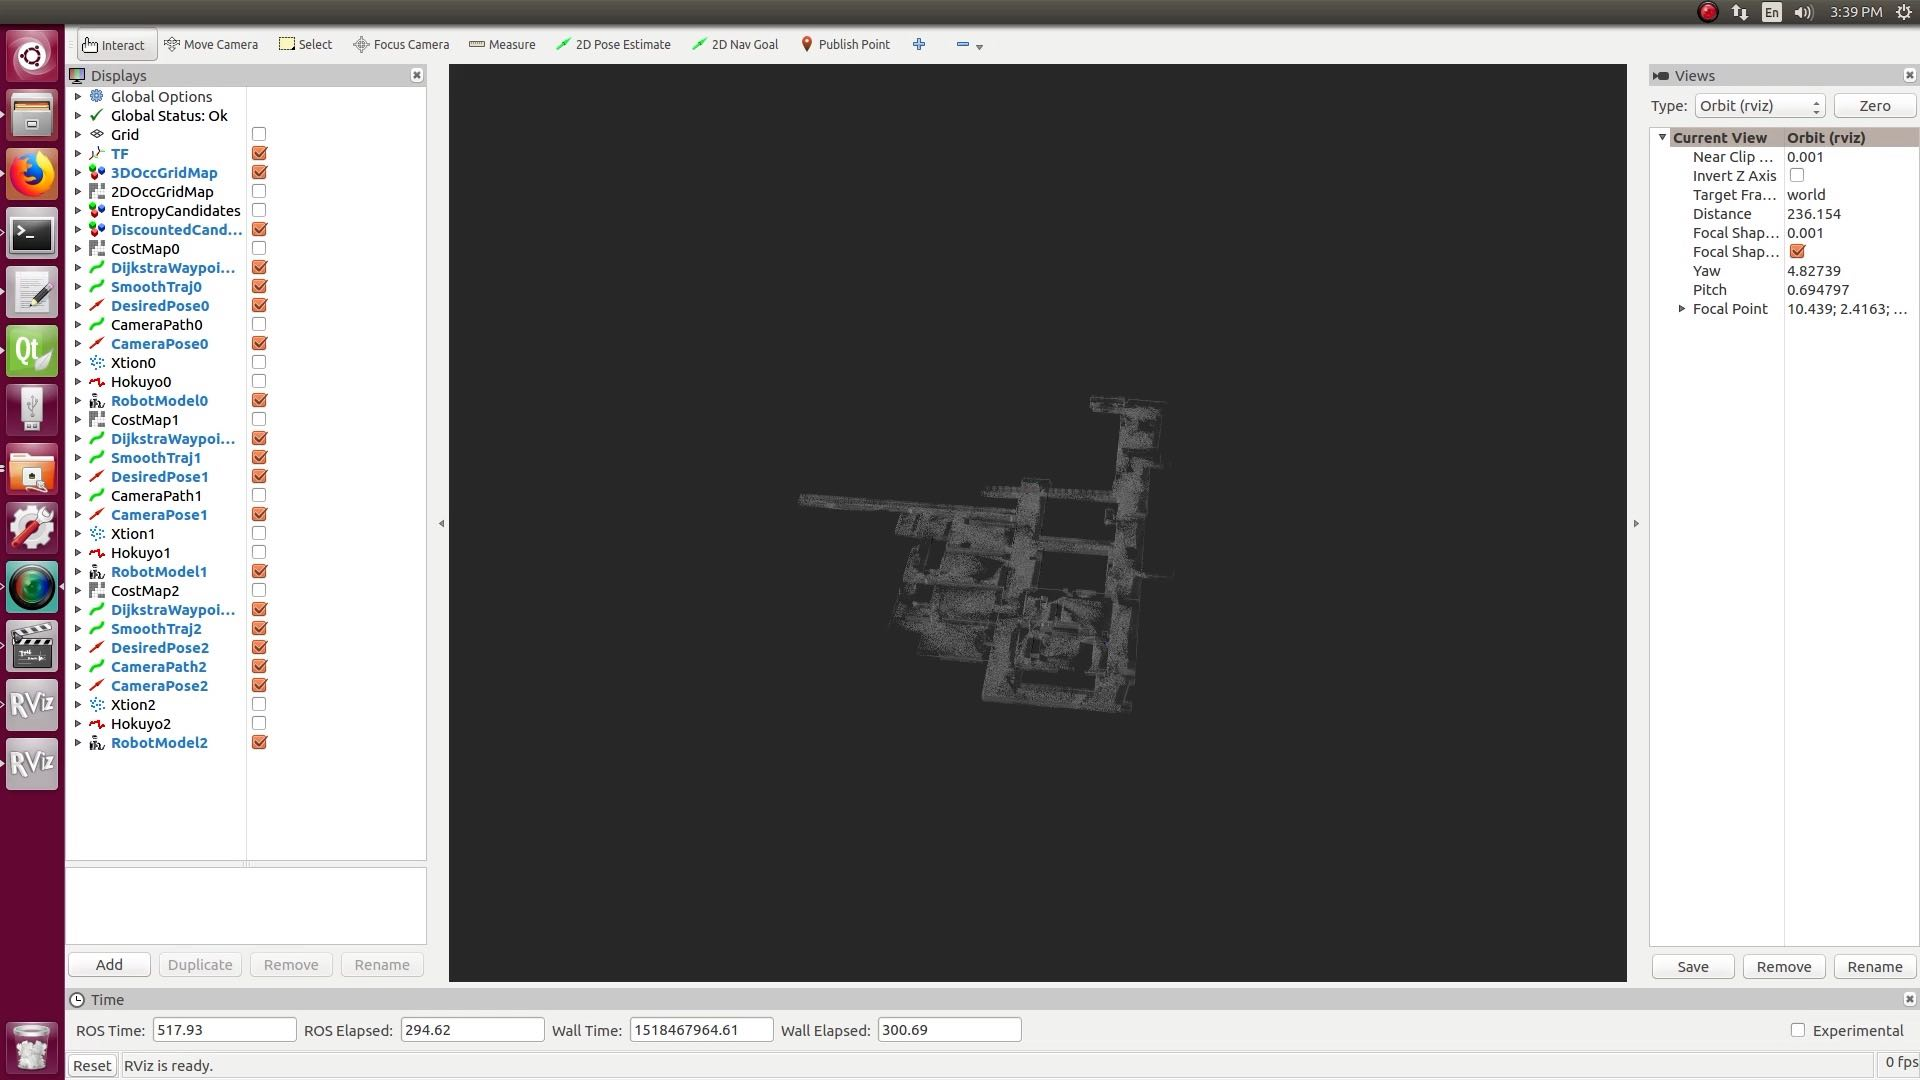
\includegraphics[trim={26cm 10cm 24cm 10cm}, clip, height=0.45\columnwidth]{multi_discount_raw_3D_5min_ss.jpg}}
		}
		\vspace*{0.025\columnwidth}
		\centerline{
			\subfigure[$6$ min]{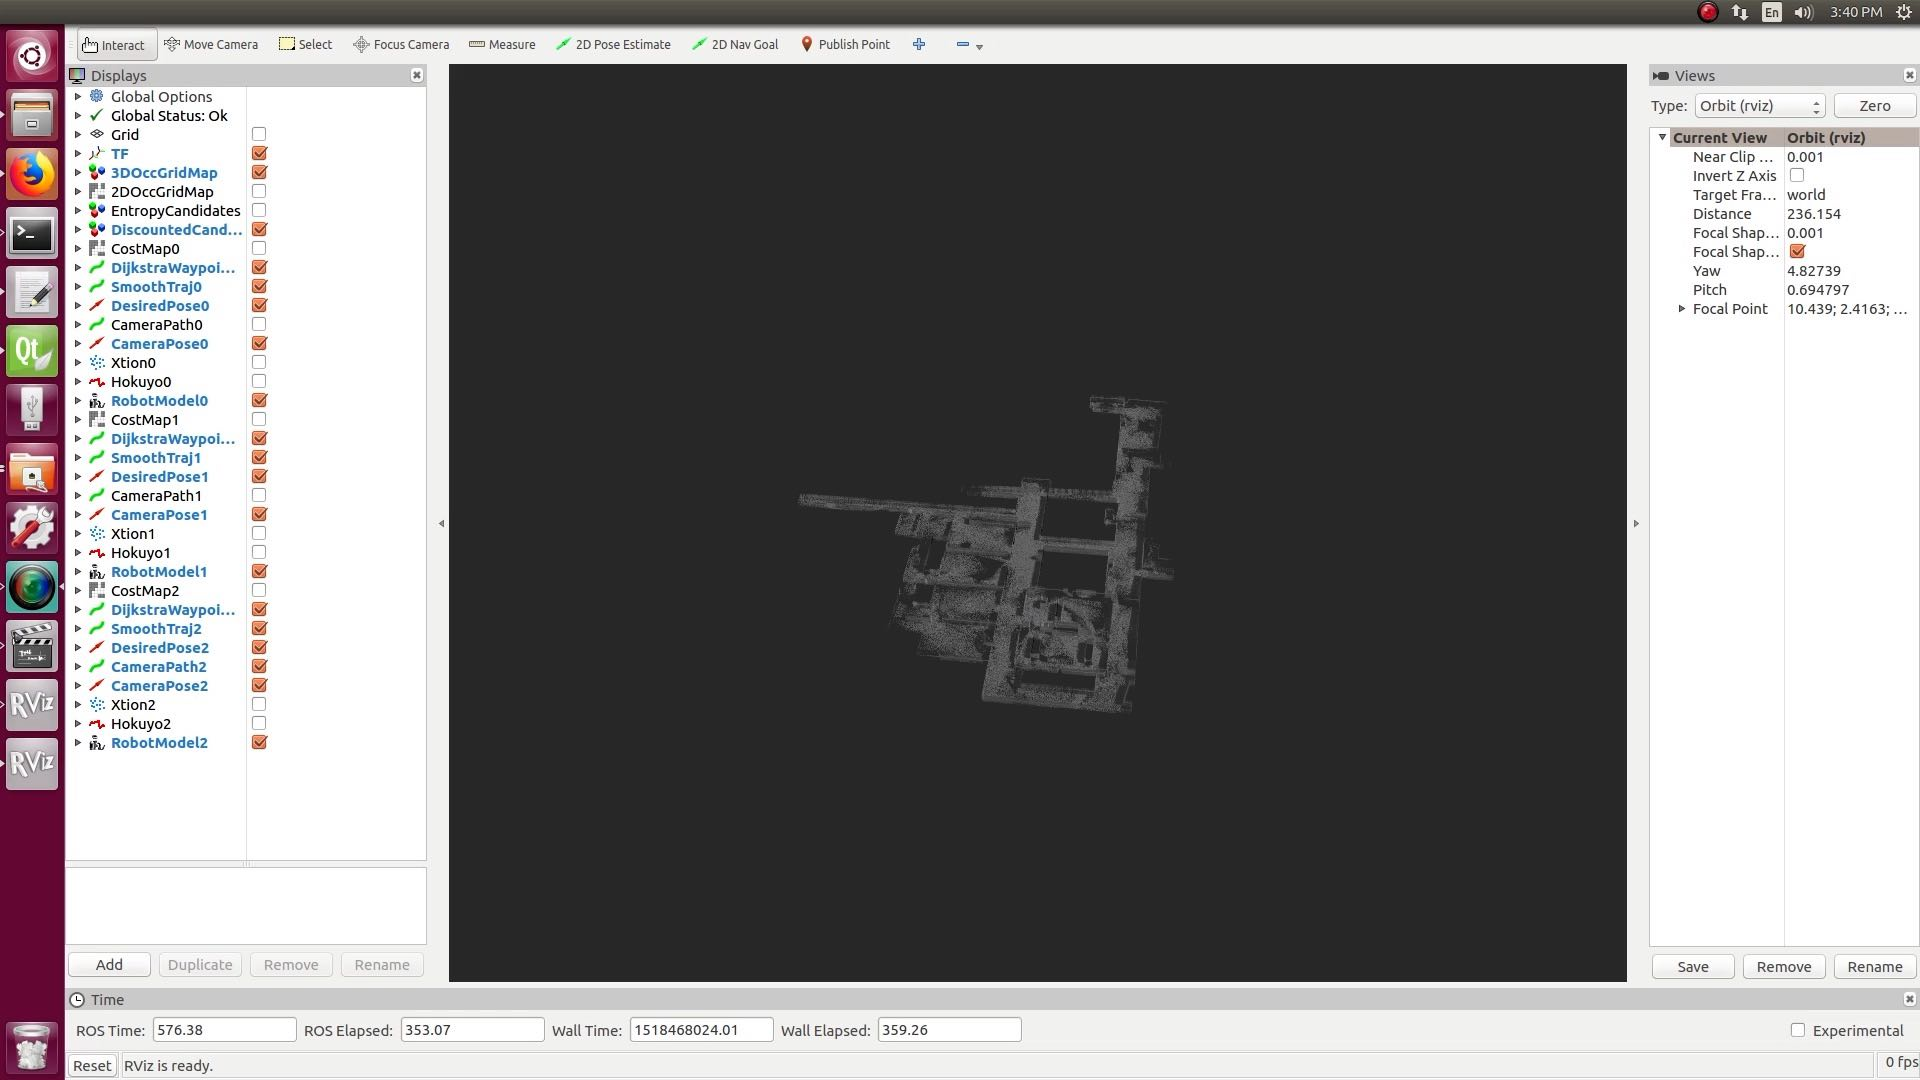
\includegraphics[trim={26cm 10cm 24cm 10cm}, clip, height=0.45\columnwidth]{multi_discount_raw_3D_6min_ss.jpg}}
			\hspace*{0.025\columnwidth}
			\subfigure[$7$ min]{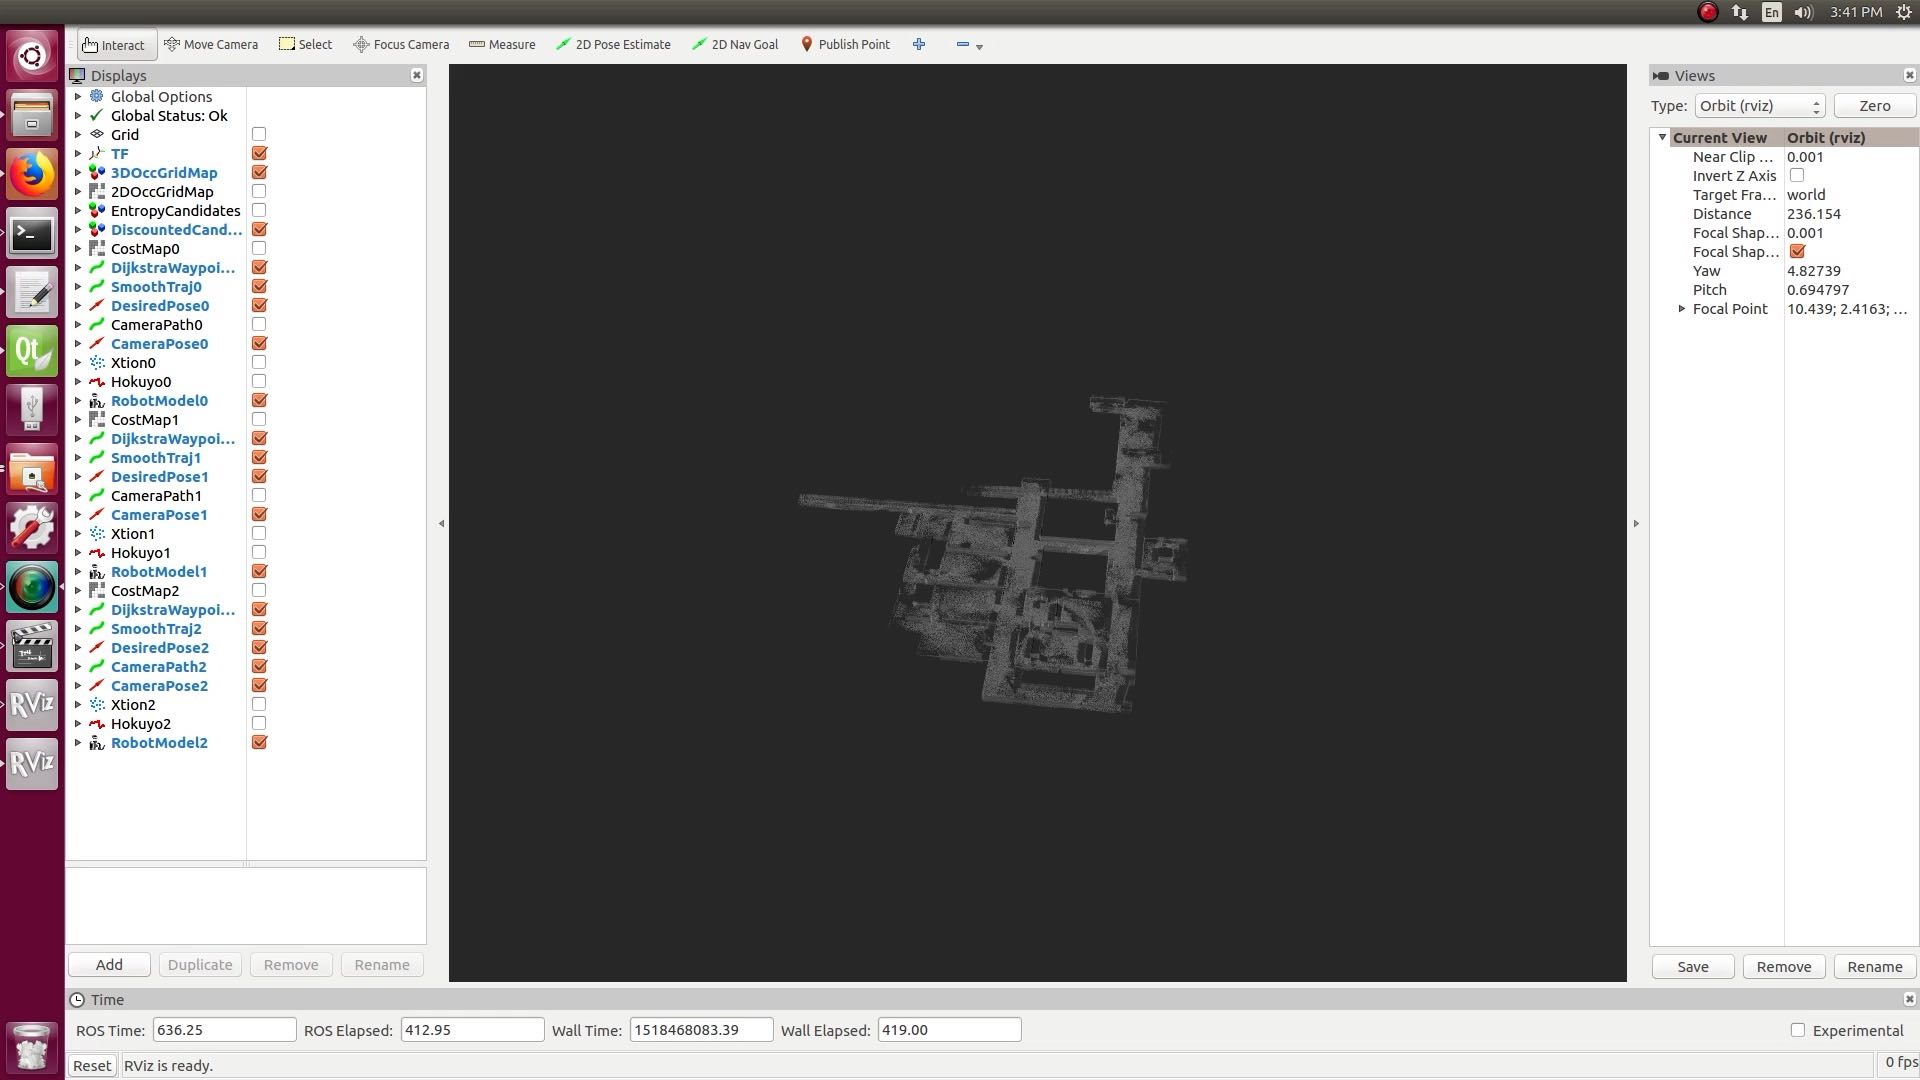
\includegraphics[trim={26cm 10cm 24cm 10cm}, clip, height=0.45\columnwidth]{multi_discount_raw_3D_7min_ss.jpg}}
		}
		\vspace*{0.025\columnwidth}
		\centerline{
			\subfigure[$8$ min]{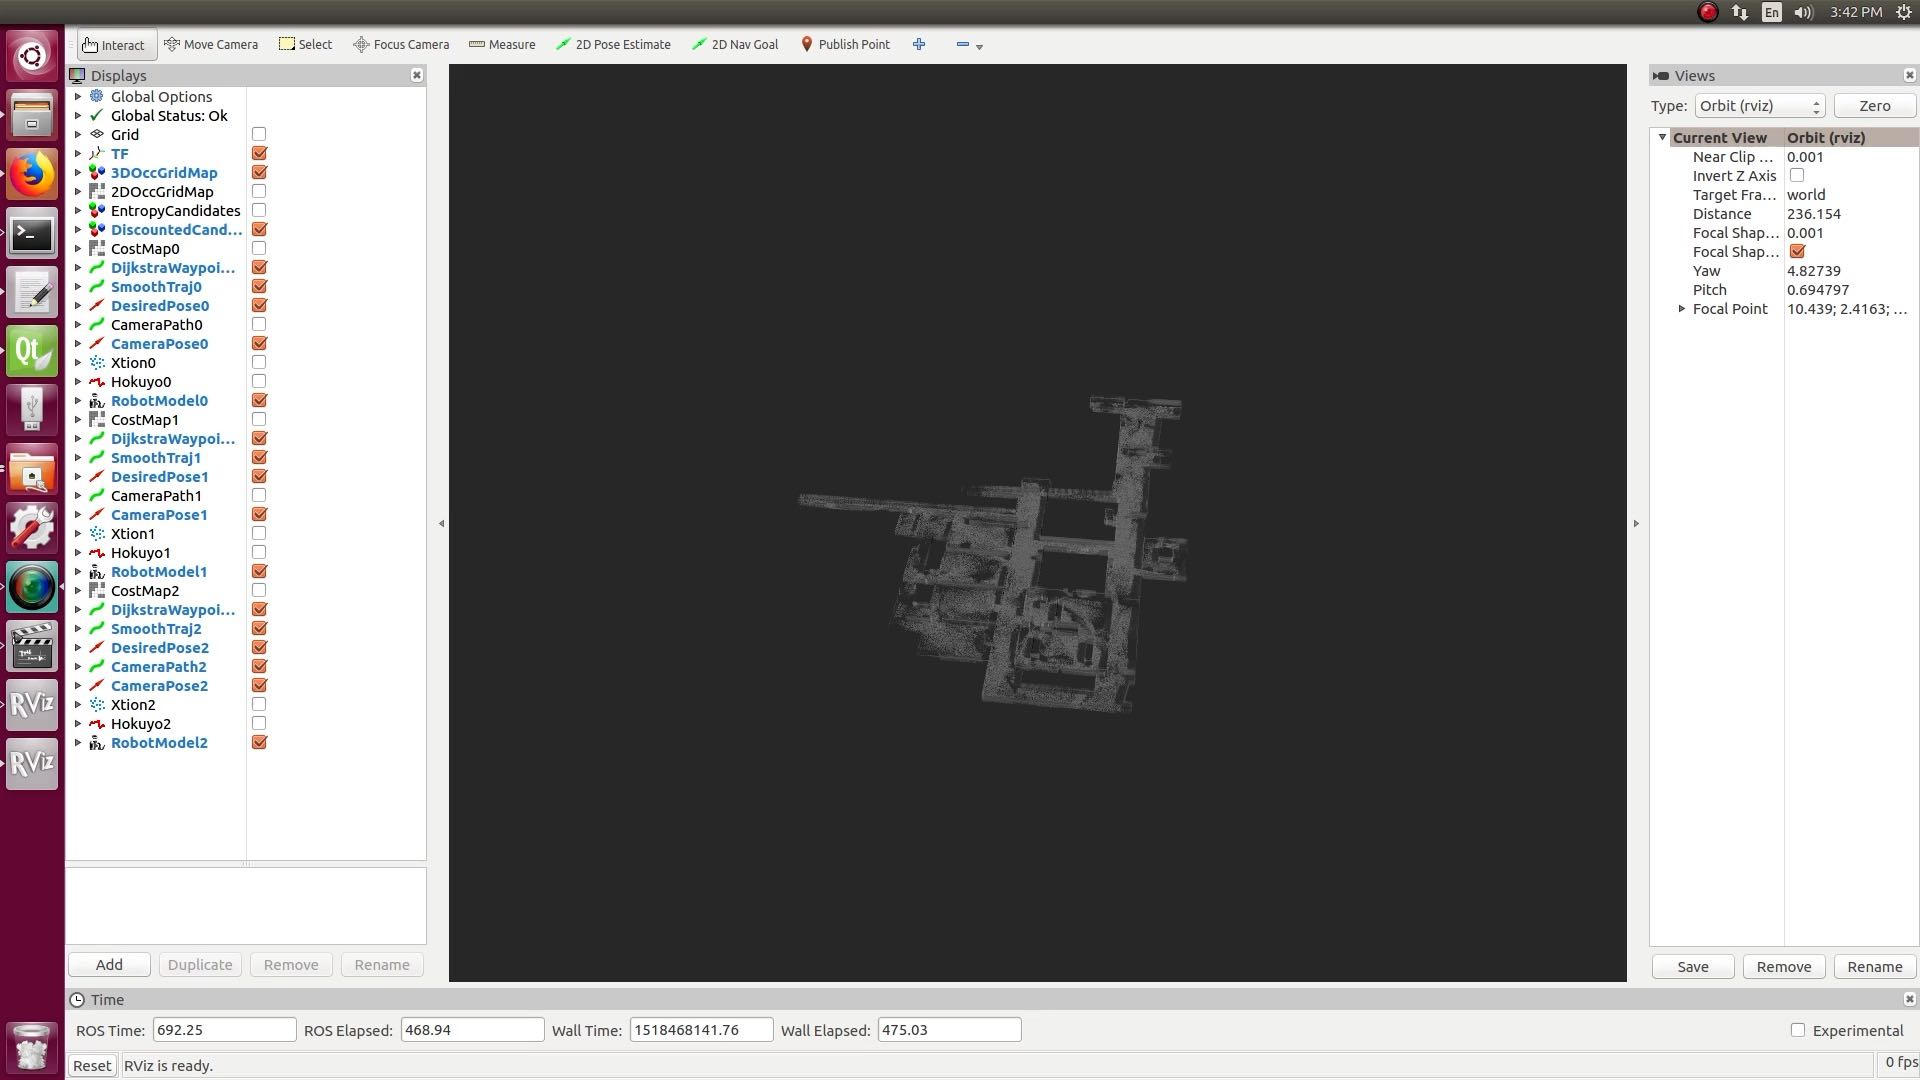
\includegraphics[trim={26cm 10cm 24cm 10cm}, clip, height=0.45\columnwidth]{multi_discount_raw_3D_8min_ss.jpg}}
			\hspace*{0.025\columnwidth}
			\subfigure[$9$ min]{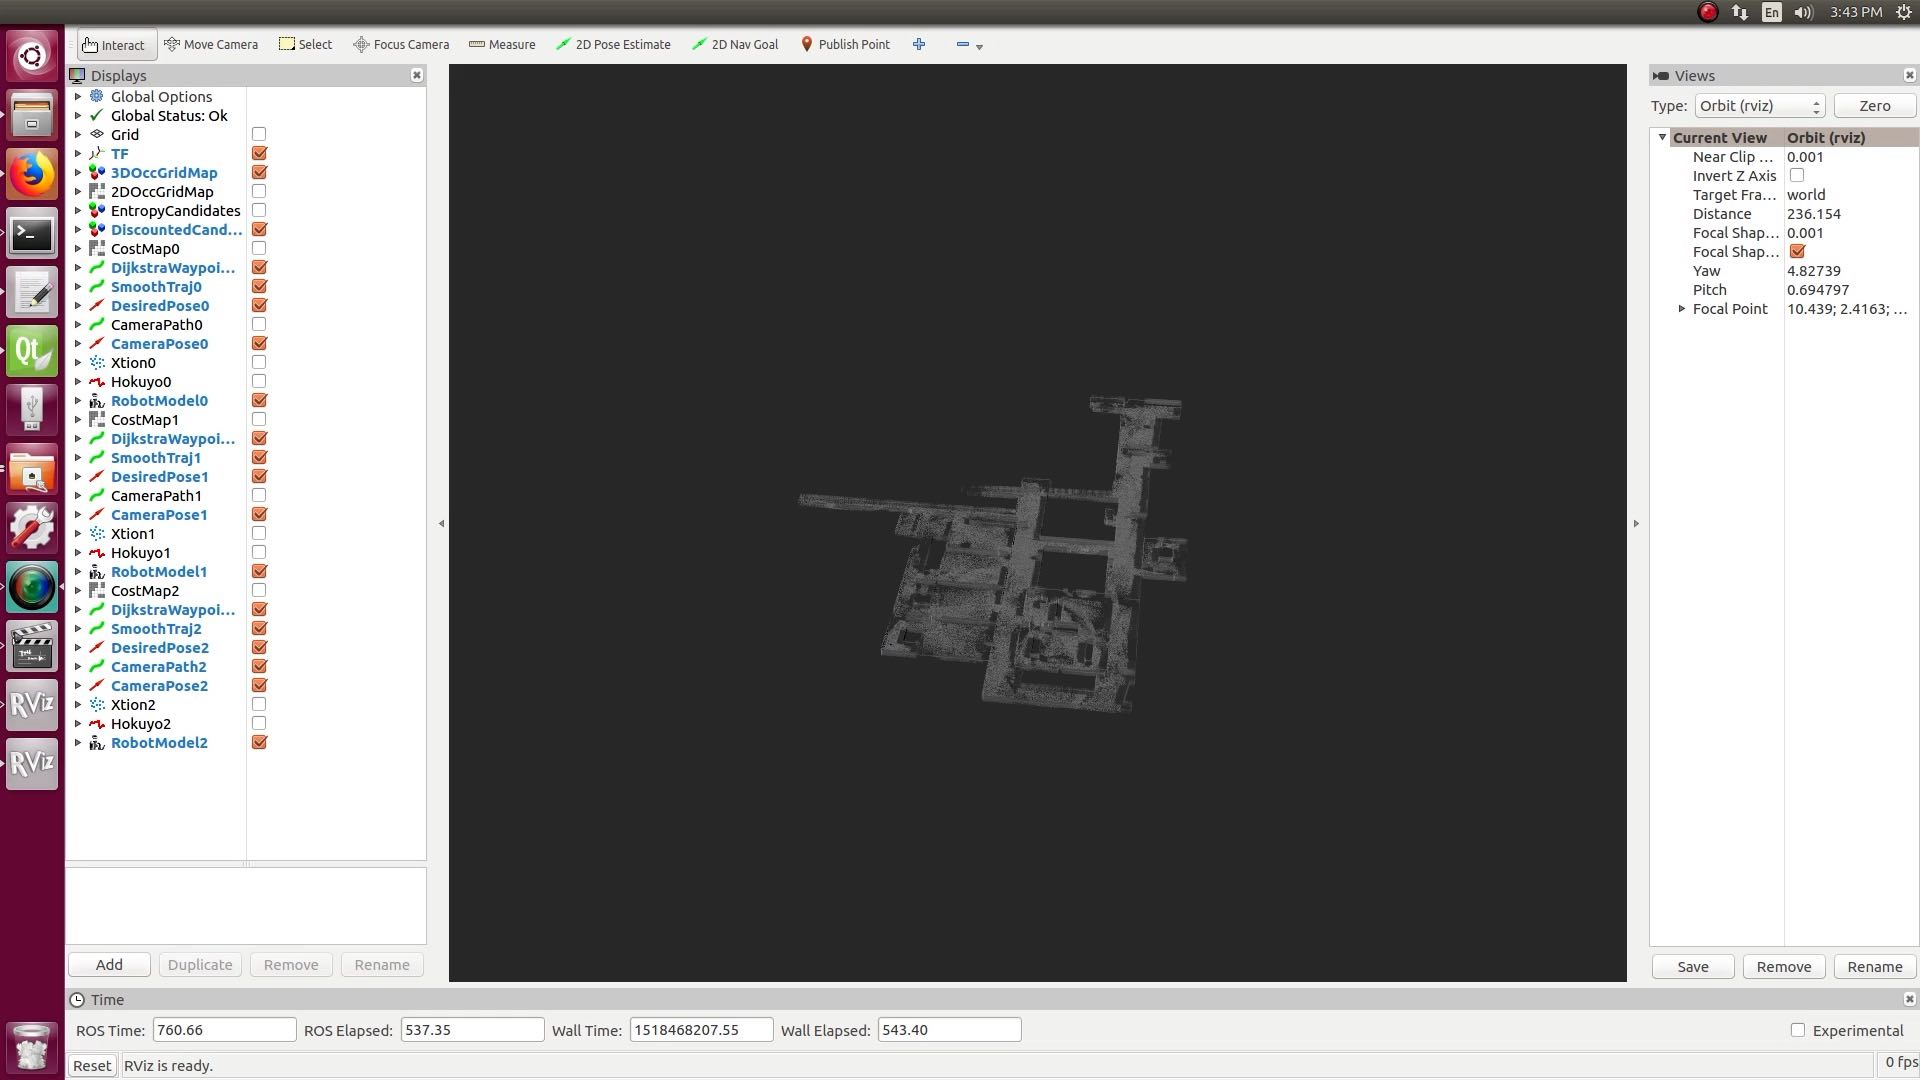
\includegraphics[trim={26cm 10cm 24cm 10cm}, clip, height=0.45\columnwidth]{multi_discount_raw_3D_9min_ss.jpg}}
		}
		\vspace*{0.025\columnwidth}
		\caption{3D Occupancy Grid Map of SEH Second Floor}
			\label{fig:sim3DMap}
	\end{figure}
	
	\begin{figure}
	% trim={<left> <lower> <right> <upper>}
		\centerline{
			\subfigure[$0$ min]{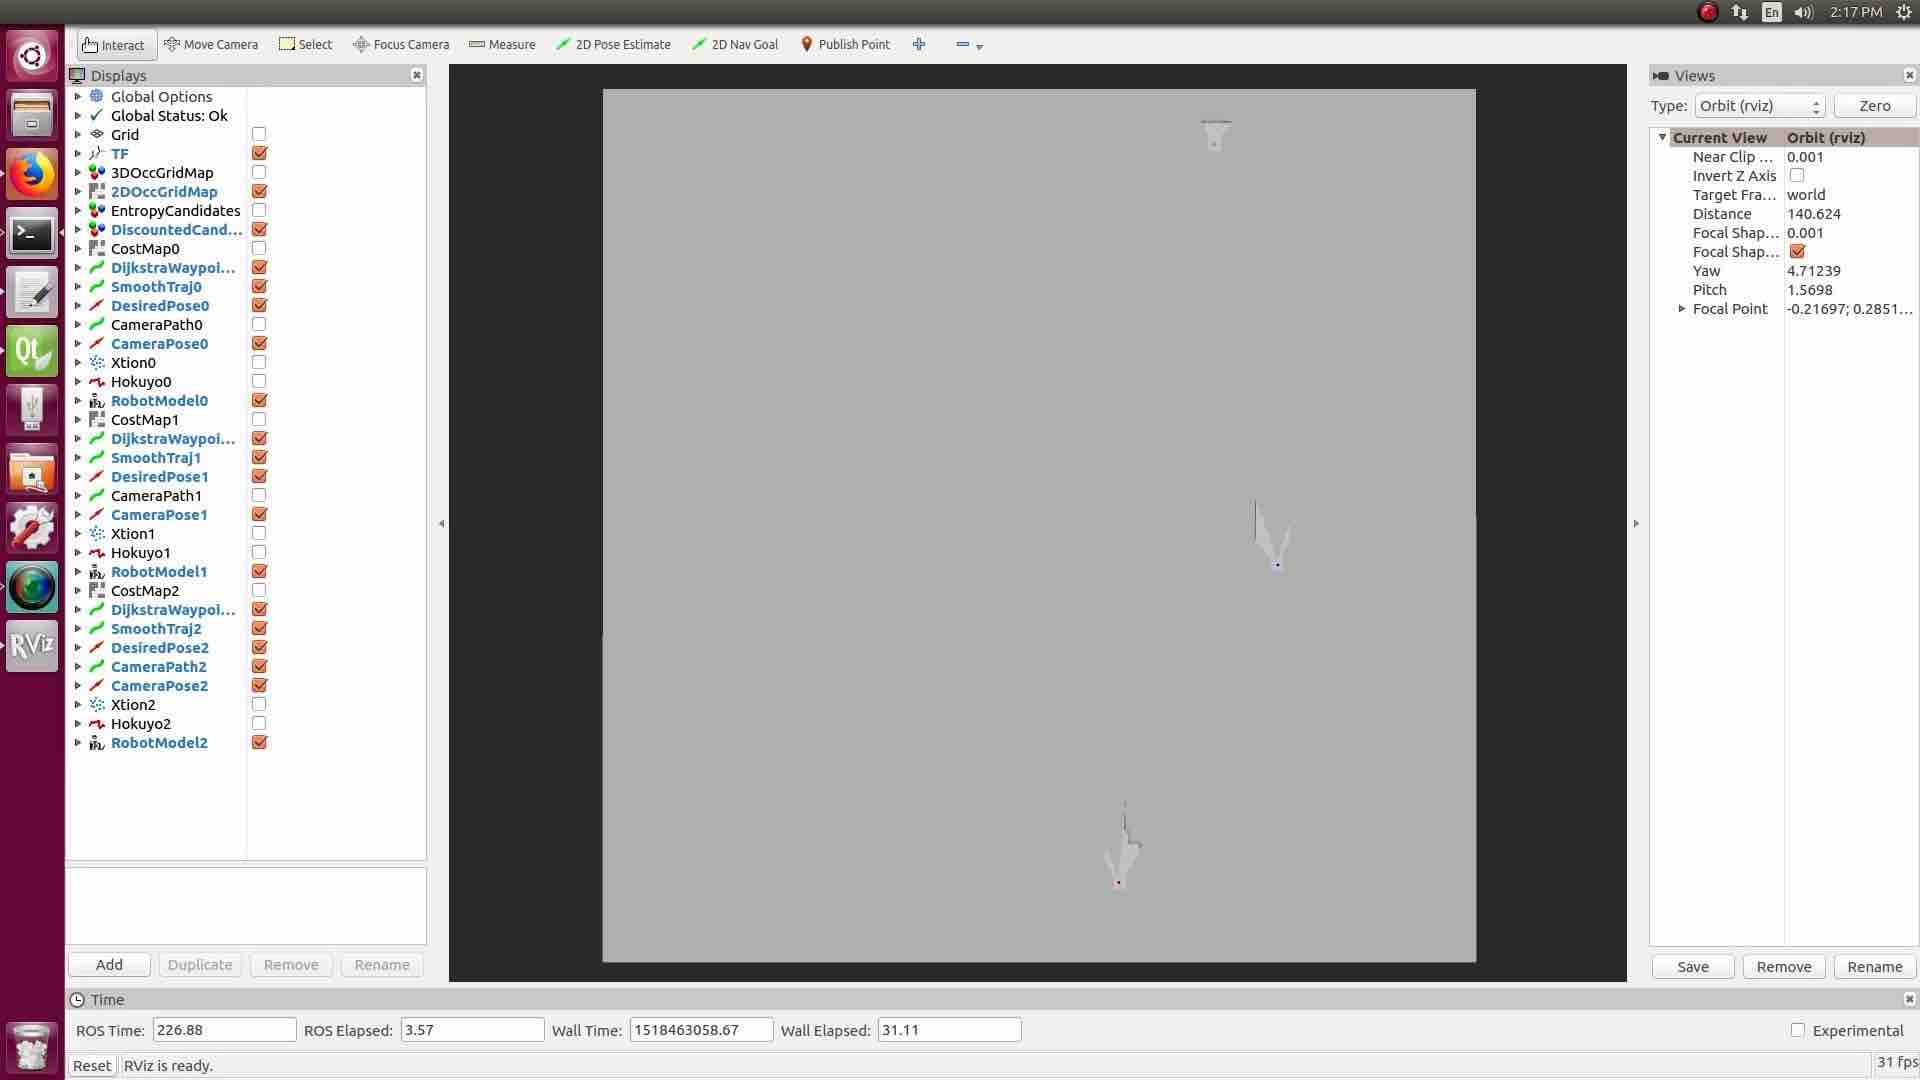
\includegraphics[trim={22cm 5cm 16cm 3.5cm}, clip, height=0.45\columnwidth]{multi_discount_raw_2D_0min_ss.jpg}}
			\hspace*{0.025\columnwidth}
			\subfigure[$1$ min]{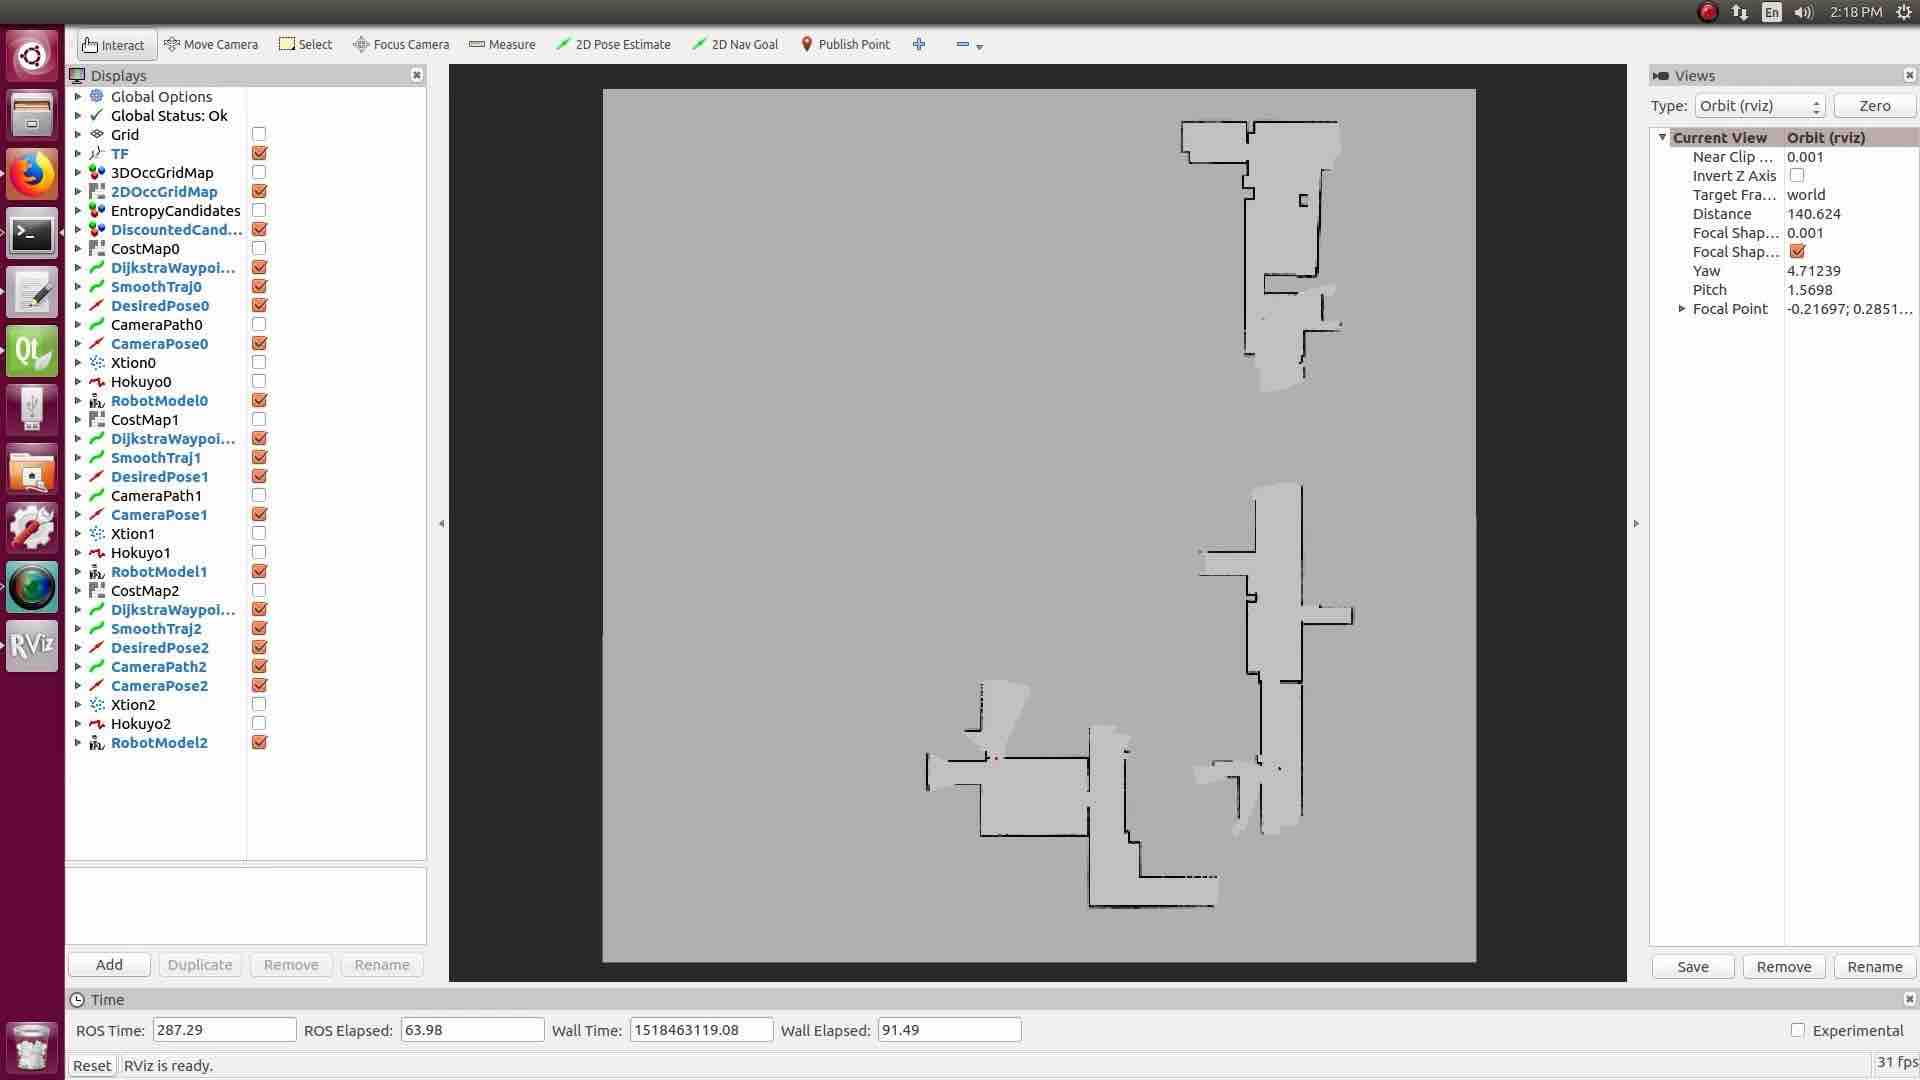
\includegraphics[trim={22cm 5cm 16cm 3.5cm}, clip, height=0.45\columnwidth]{multi_discount_raw_2D_1min_ss.jpg}}
		}
		\vspace*{0.025\columnwidth}
		\centerline{
			\subfigure[$2$ min]{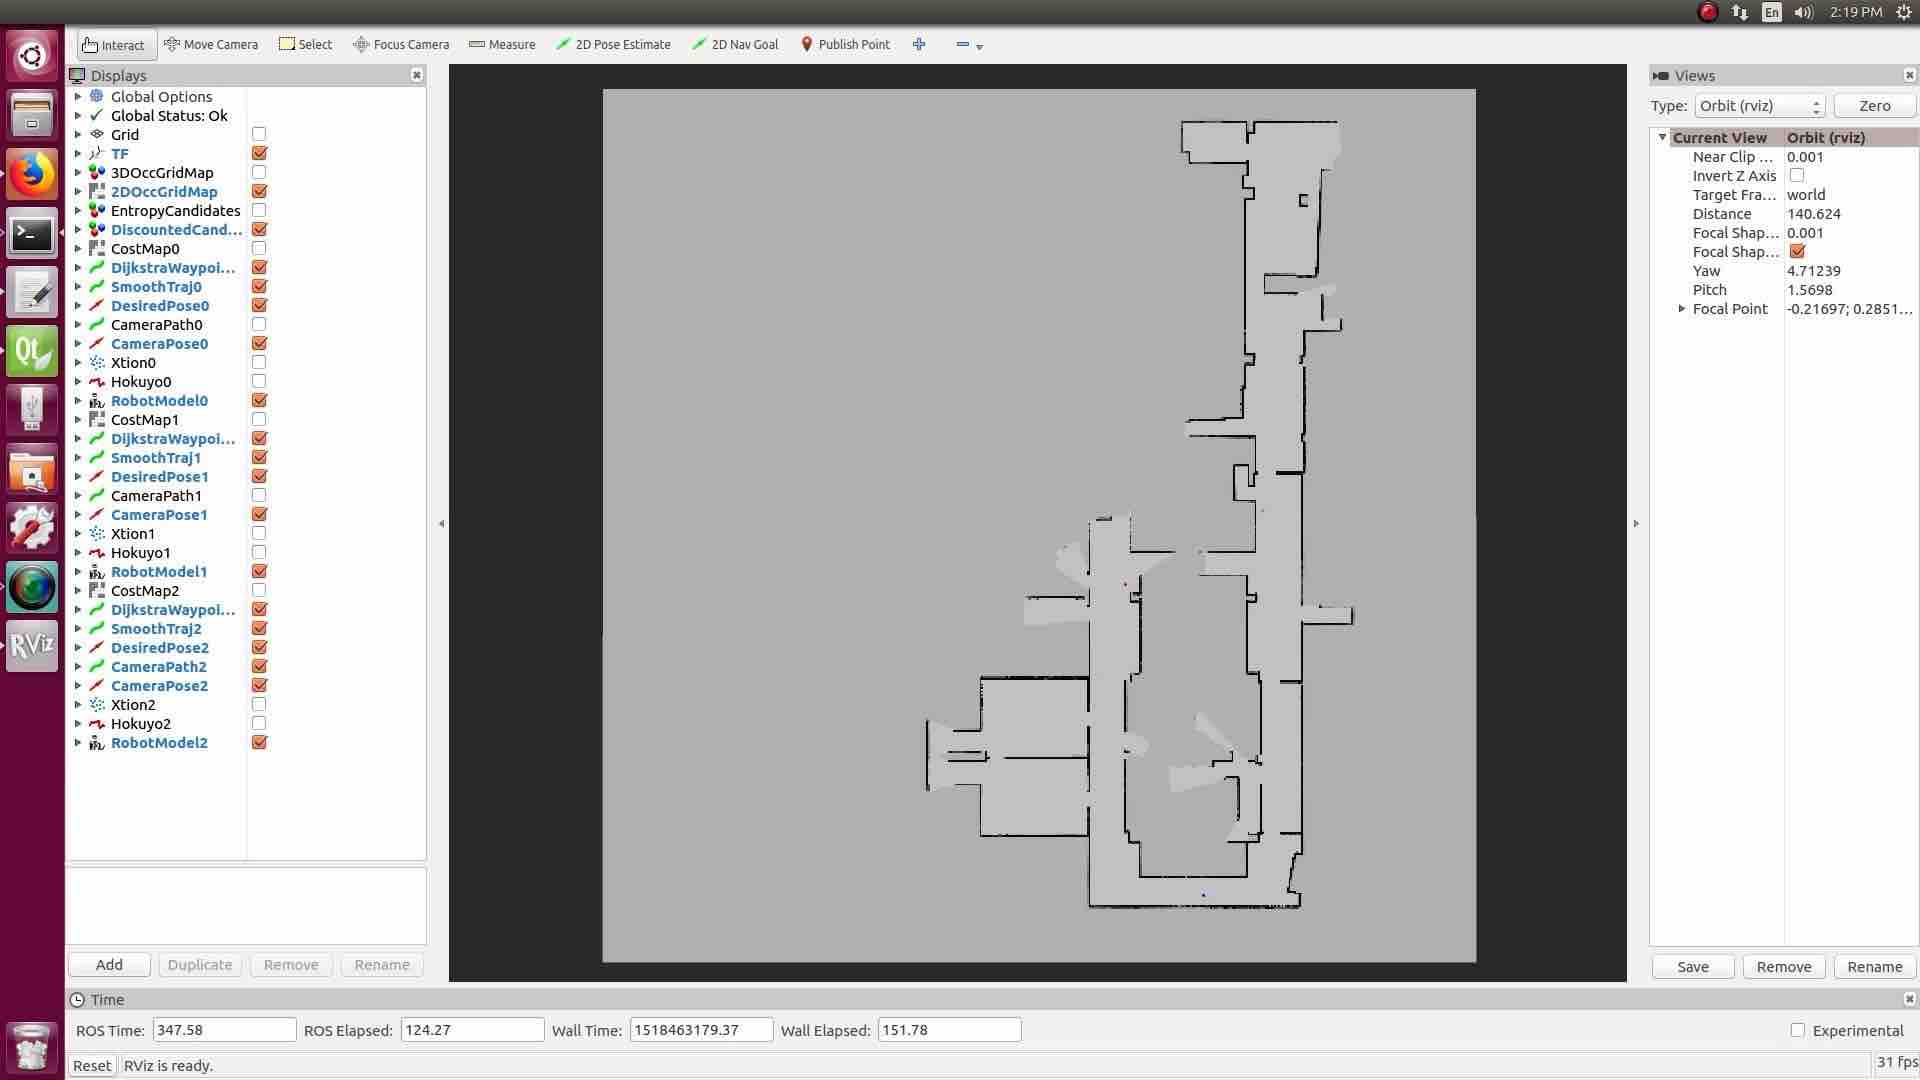
\includegraphics[trim={22cm 5cm 16cm 3.5cm}, clip, height=0.45\columnwidth]{multi_discount_raw_2D_2min_ss.jpg}}
			\hspace*{0.025\columnwidth}
			\subfigure[$3$ min]{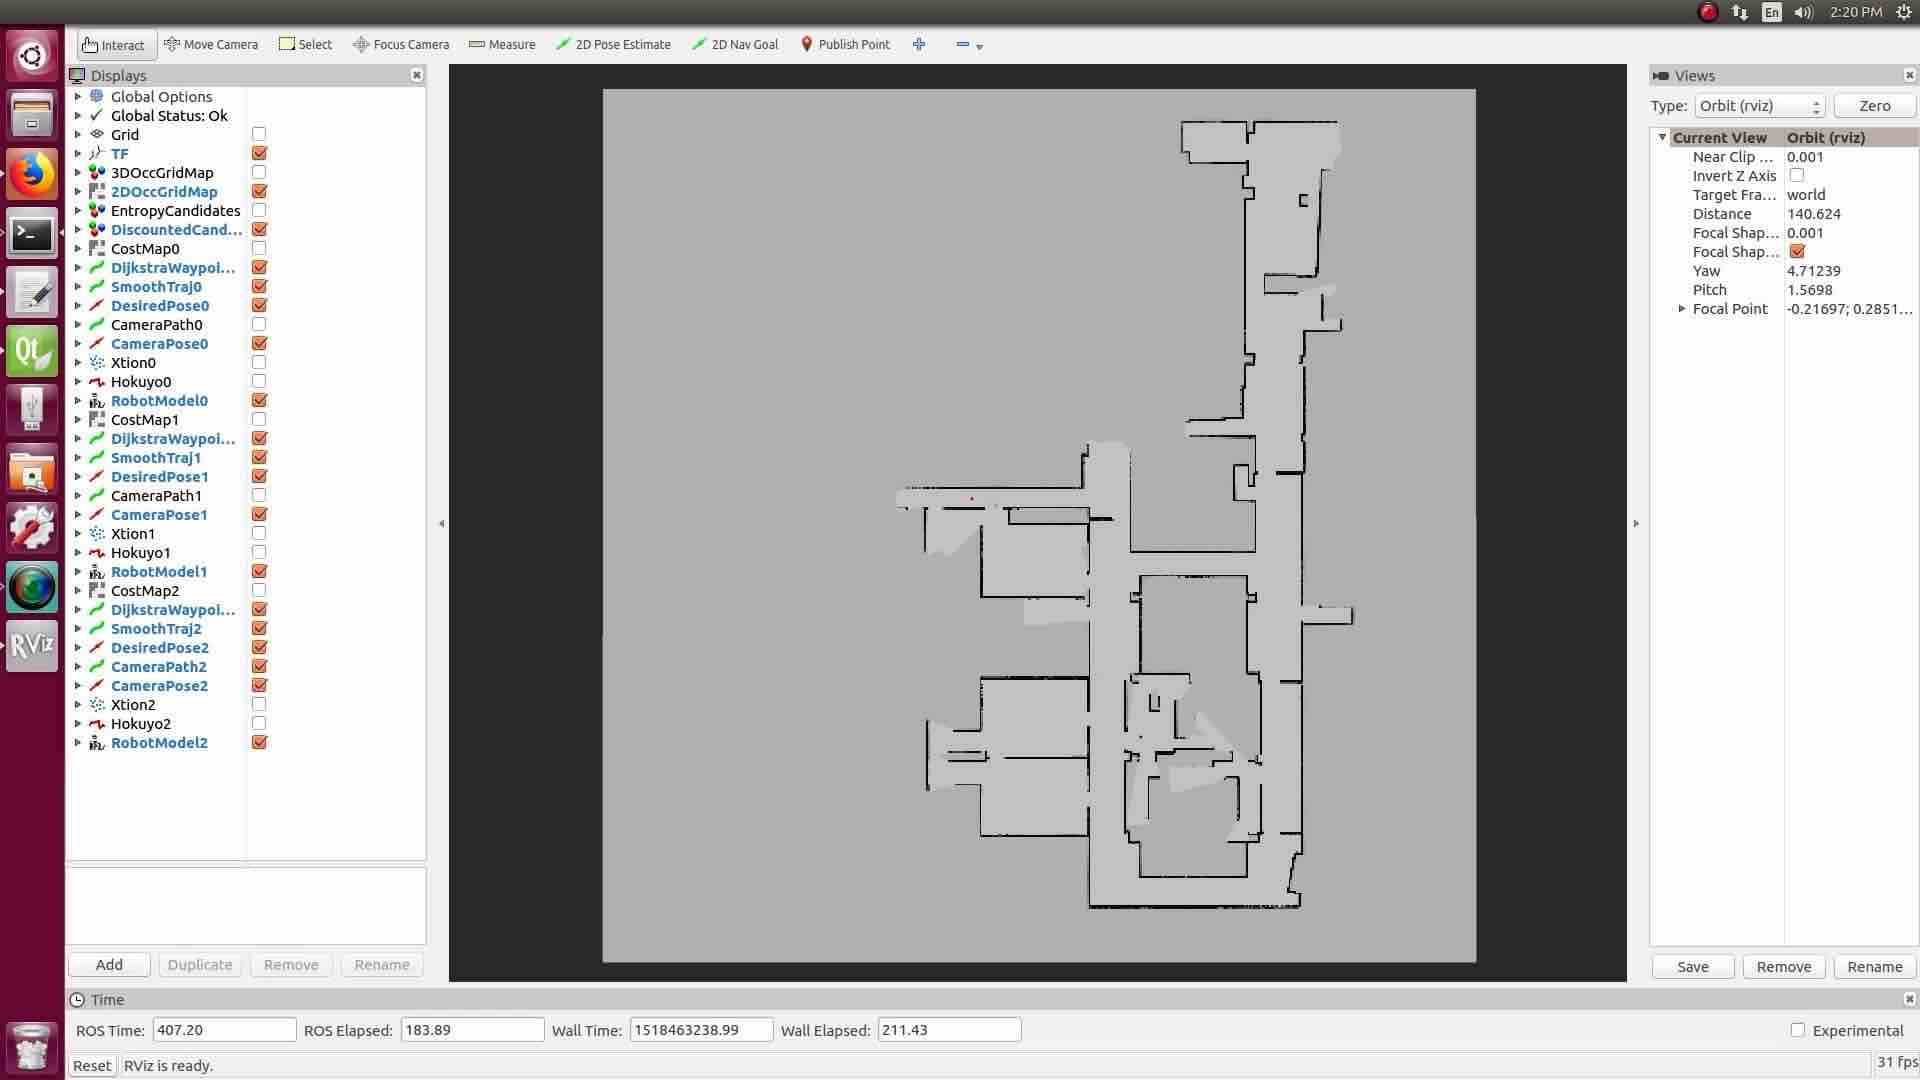
\includegraphics[trim={22cm 5cm 16cm 3.5cm}, clip, height=0.45\columnwidth]{multi_discount_raw_2D_3min_ss.jpg}}
		}
		\vspace*{0.025\columnwidth}
		\centerline{
			\subfigure[$4$ min]{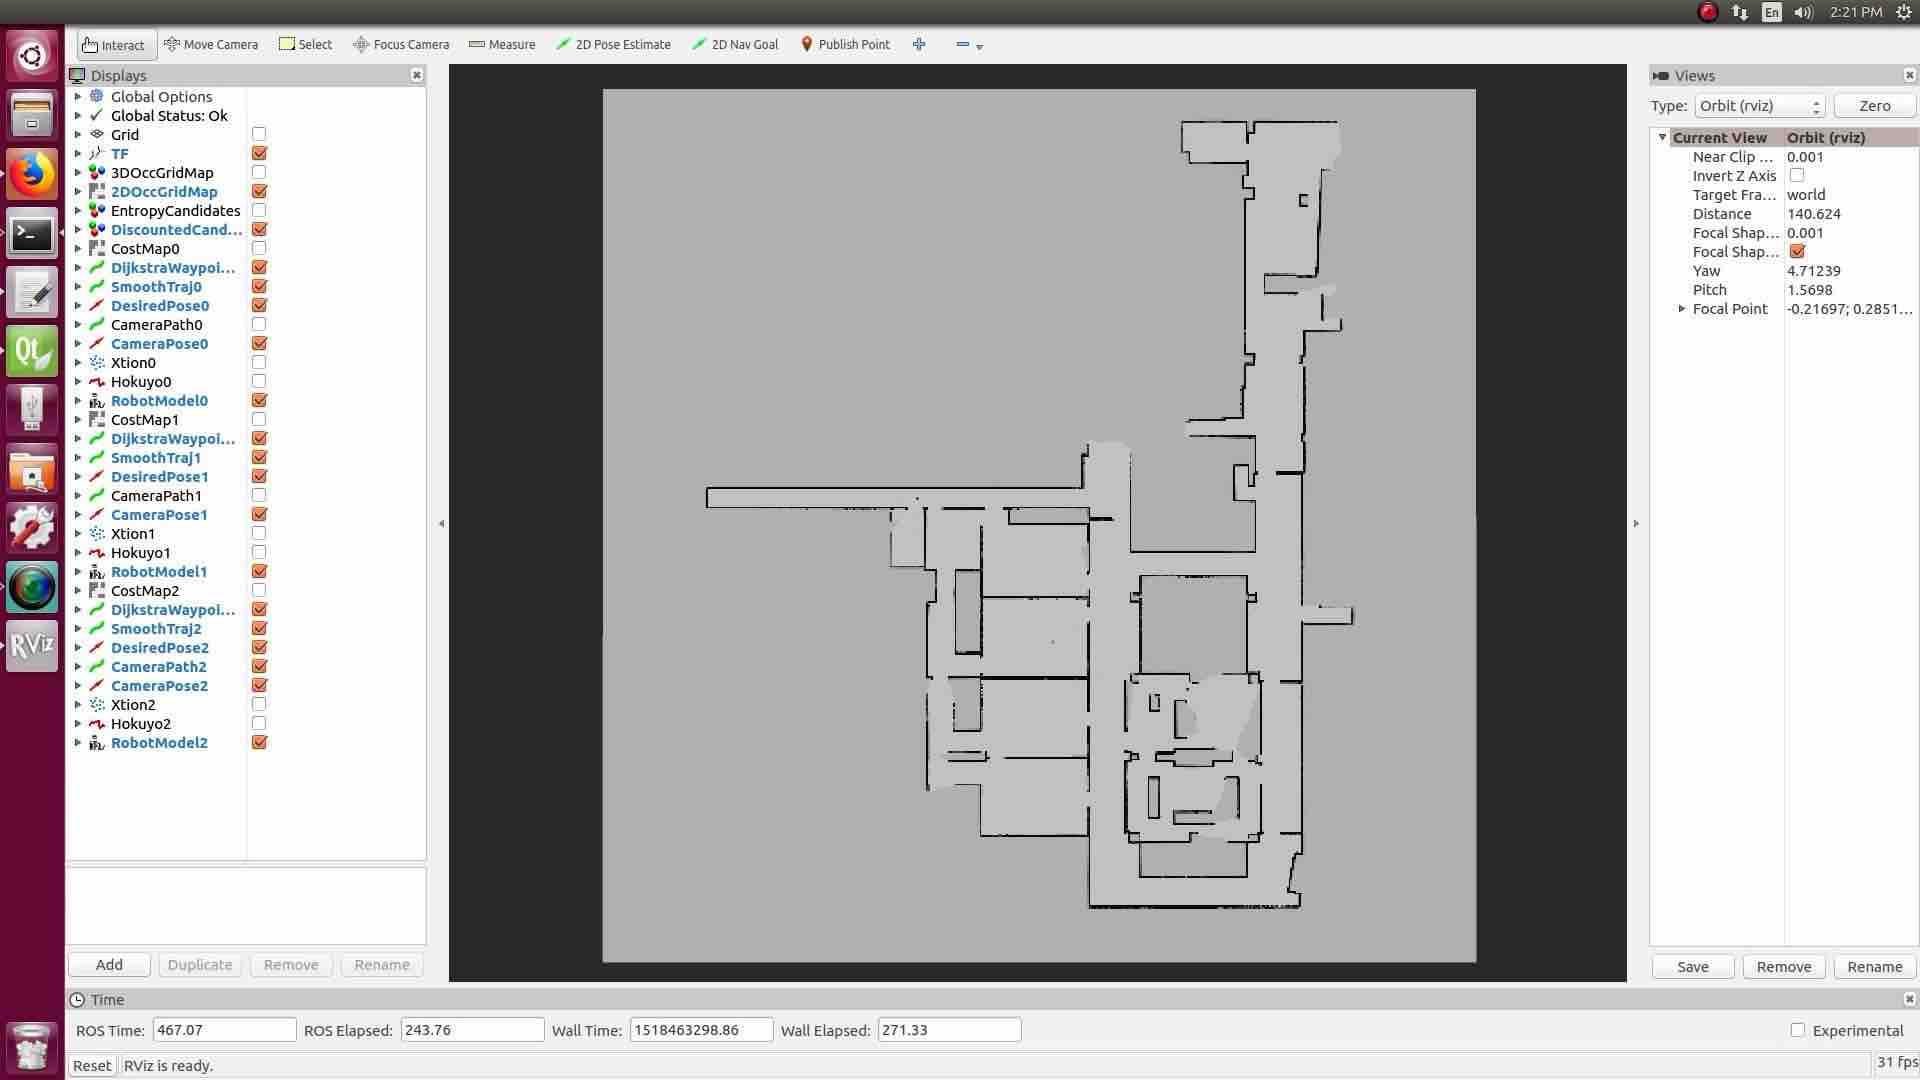
\includegraphics[trim={22cm 5cm 16cm 3.5cm}, clip, height=0.45\columnwidth]{multi_discount_raw_2D_4min_ss.jpg}}
			\hspace*{0.025\columnwidth}
			\subfigure[$5$ min]{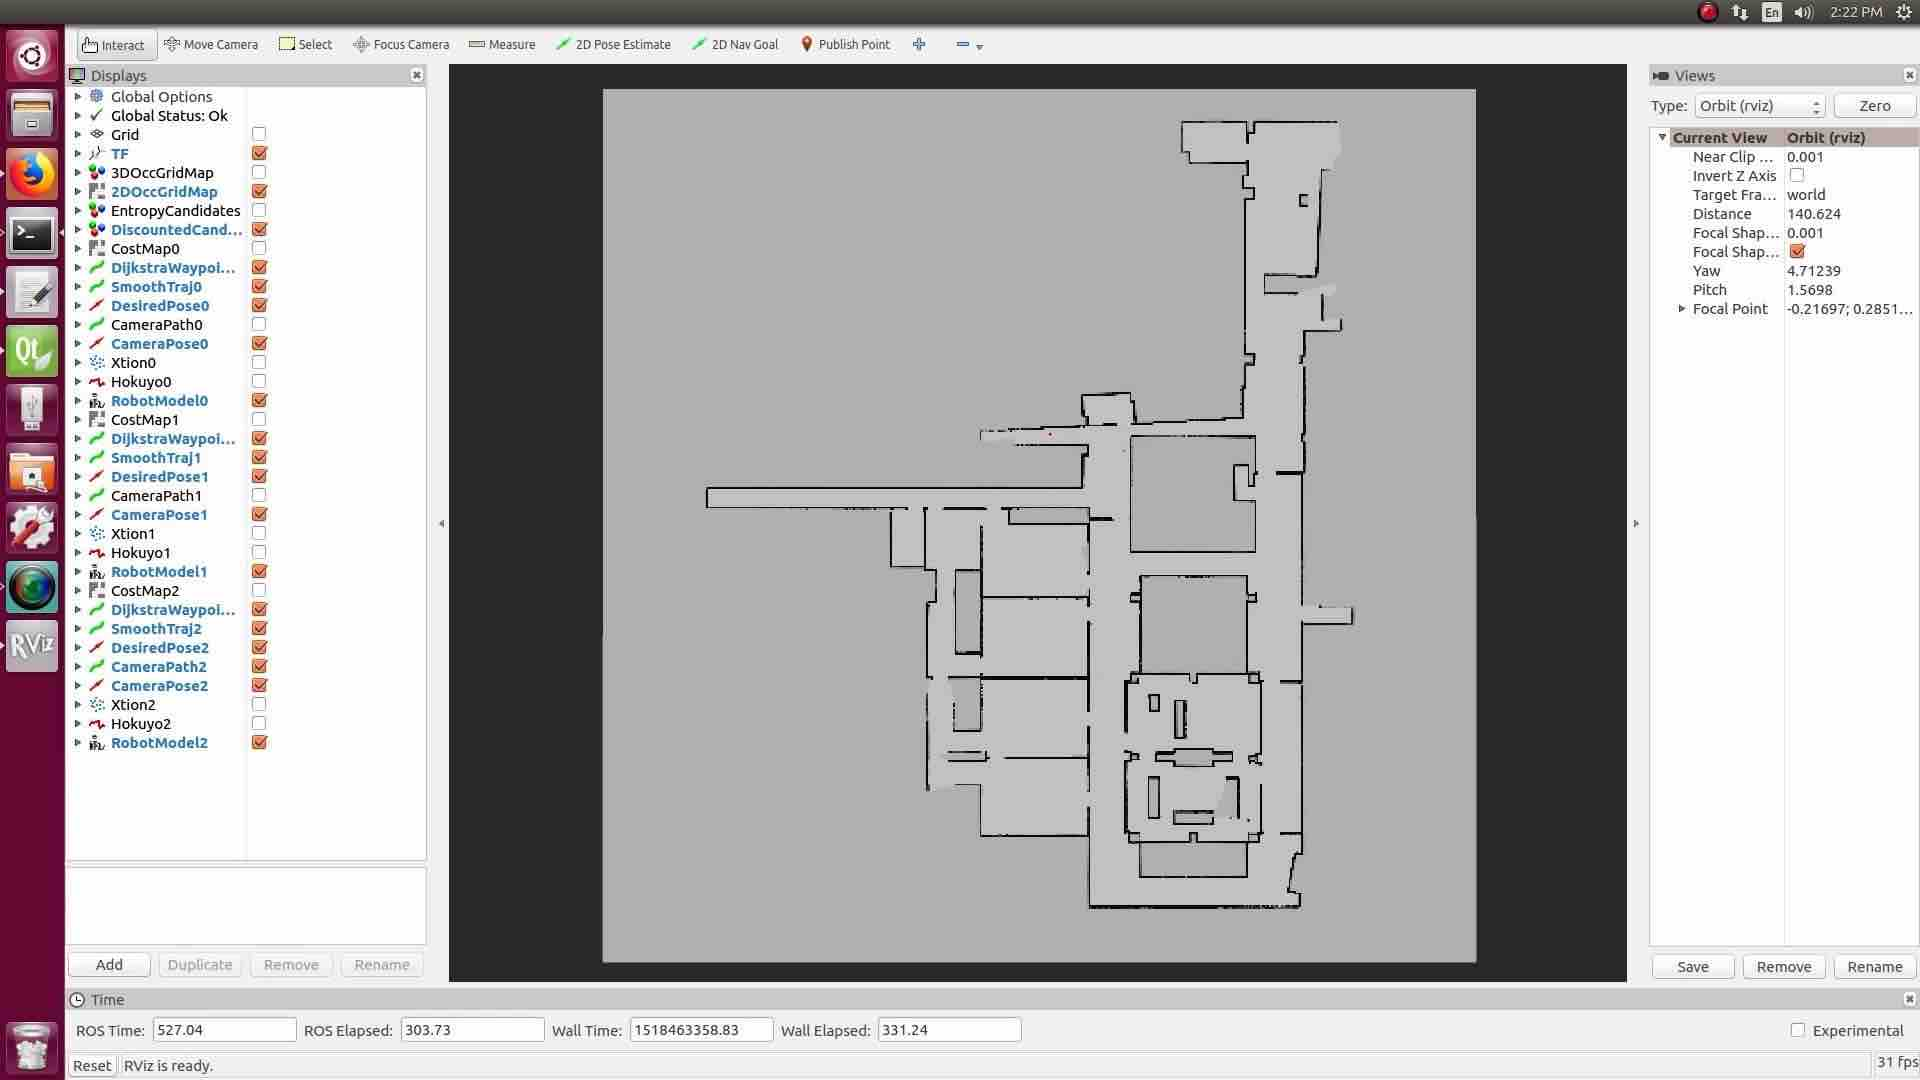
\includegraphics[trim={22cm 5cm 16cm 3.5cm}, clip, height=0.45\columnwidth]{multi_discount_raw_2D_5min_ss.jpg}}
		}
		\vspace*{0.025\columnwidth}
		\centerline{
			\subfigure[$6$ min]{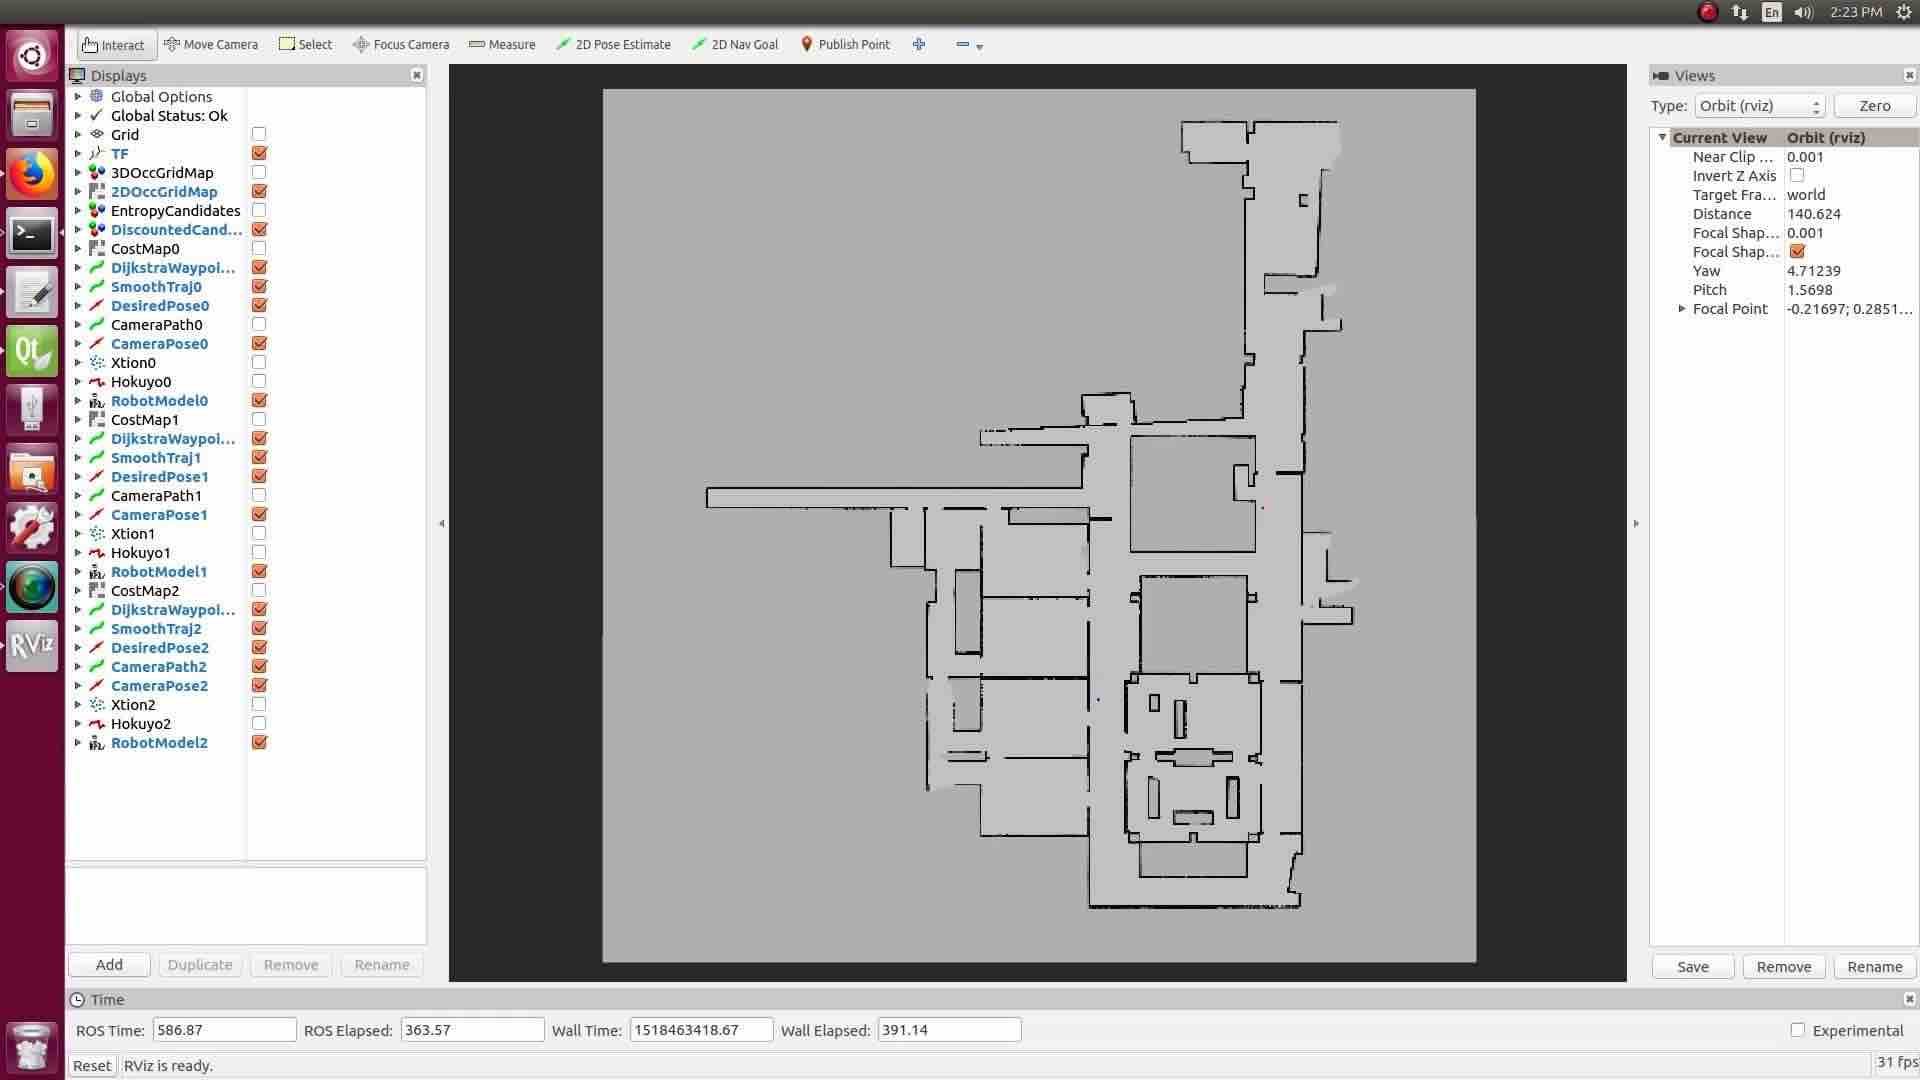
\includegraphics[trim={22cm 5cm 16cm 3.5cm}, clip, height=0.45\columnwidth]{multi_discount_raw_2D_6min_ss.jpg}}
			\hspace*{0.025\columnwidth}
			\subfigure[$7$ min]{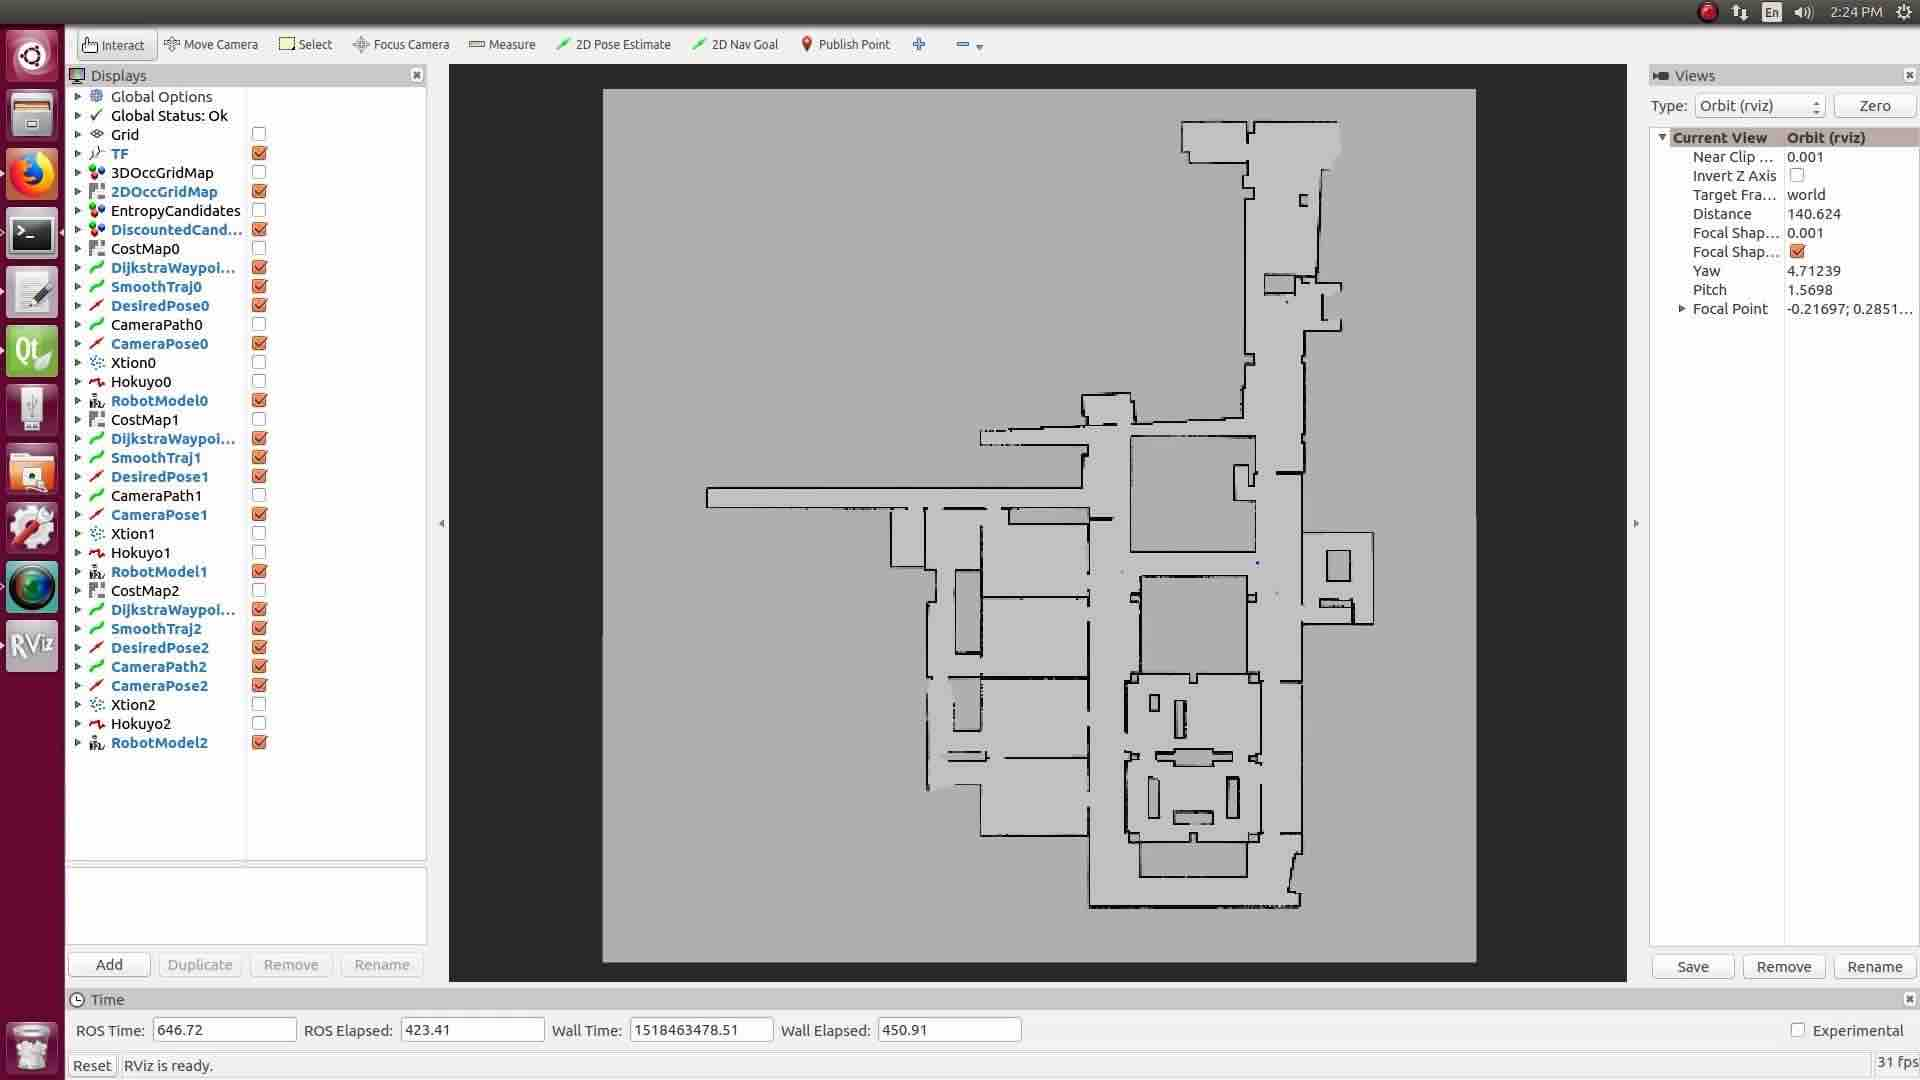
\includegraphics[trim={22cm 5cm 16cm 3.5cm}, clip, height=0.45\columnwidth]{multi_discount_raw_2D_7min_ss.jpg}}
		}
		\vspace*{0.025\columnwidth}
		\centerline{
			\subfigure[$8$ min]{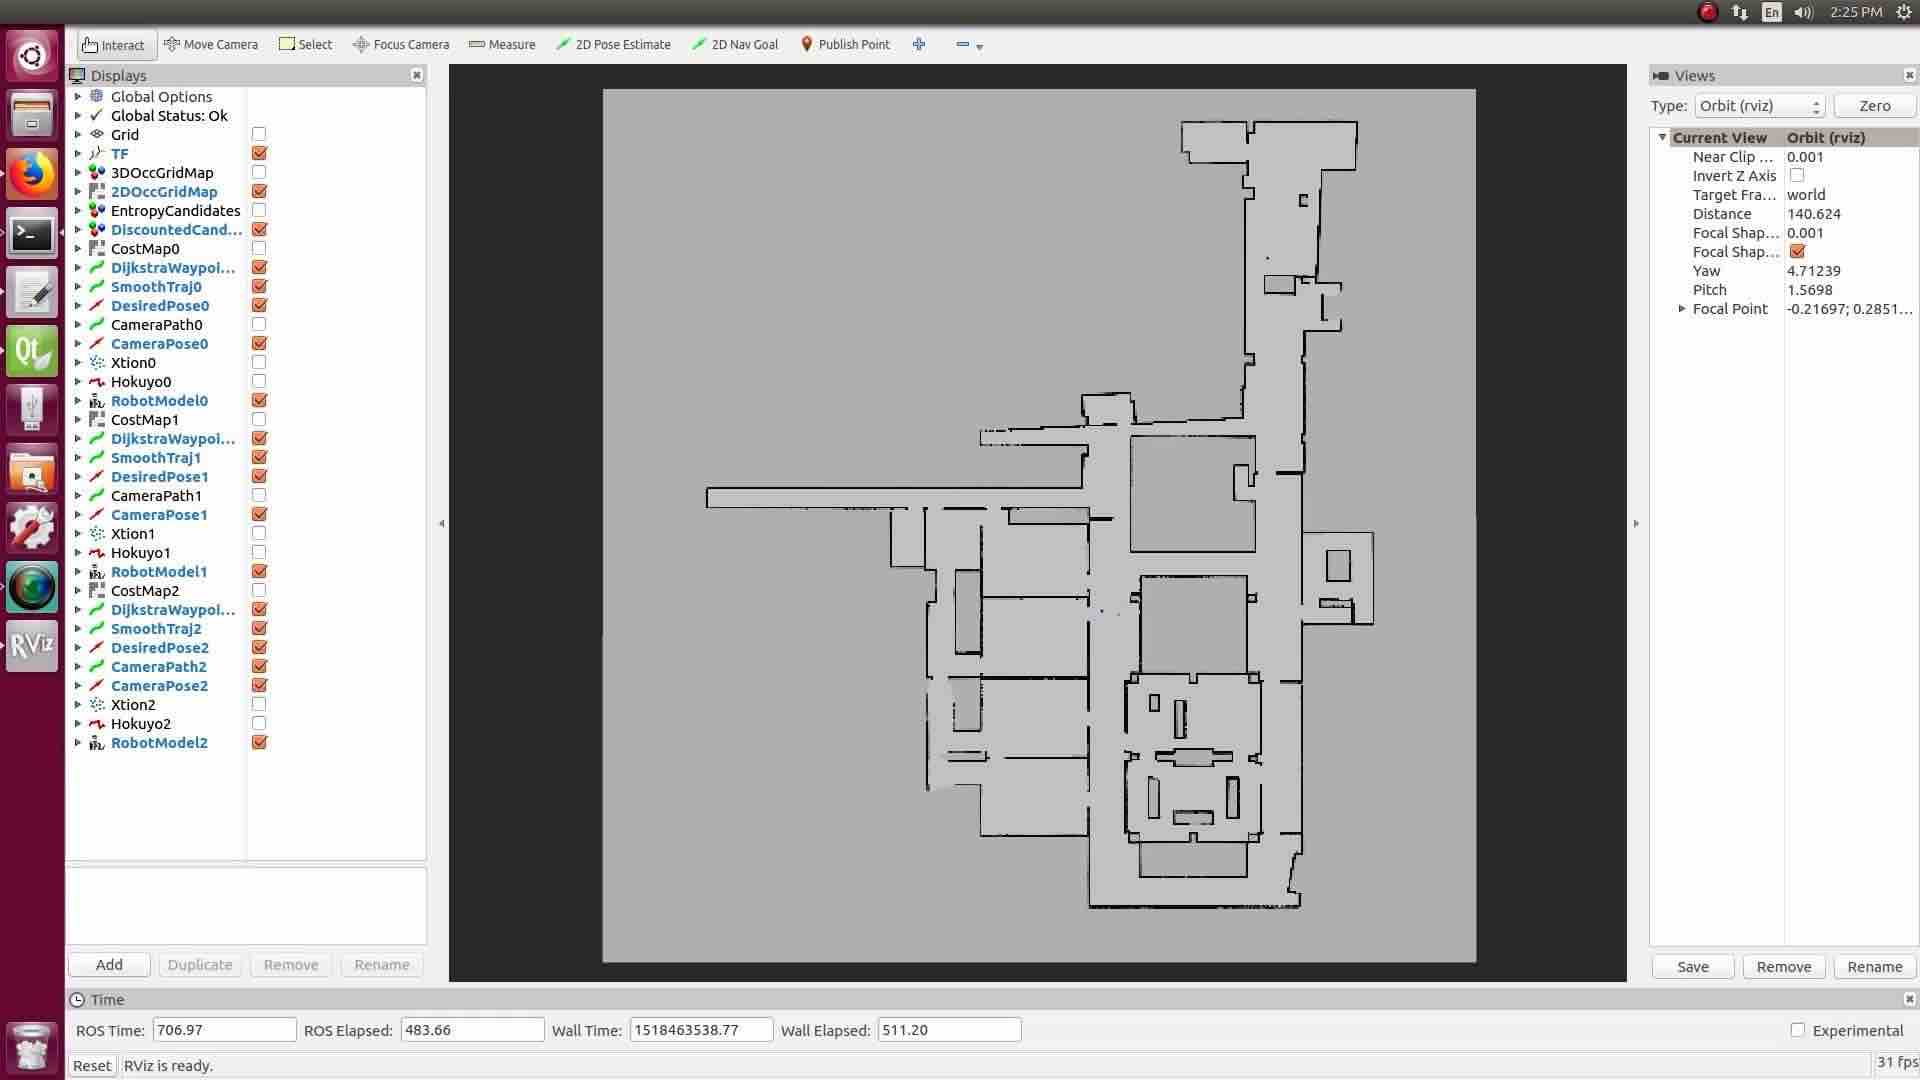
\includegraphics[trim={22cm 5cm 16cm 3.5cm}, clip, height=0.45\columnwidth]{multi_discount_raw_2D_8min_ss.jpg}}
			\hspace*{0.025\columnwidth}
			\subfigure[$9$ min]{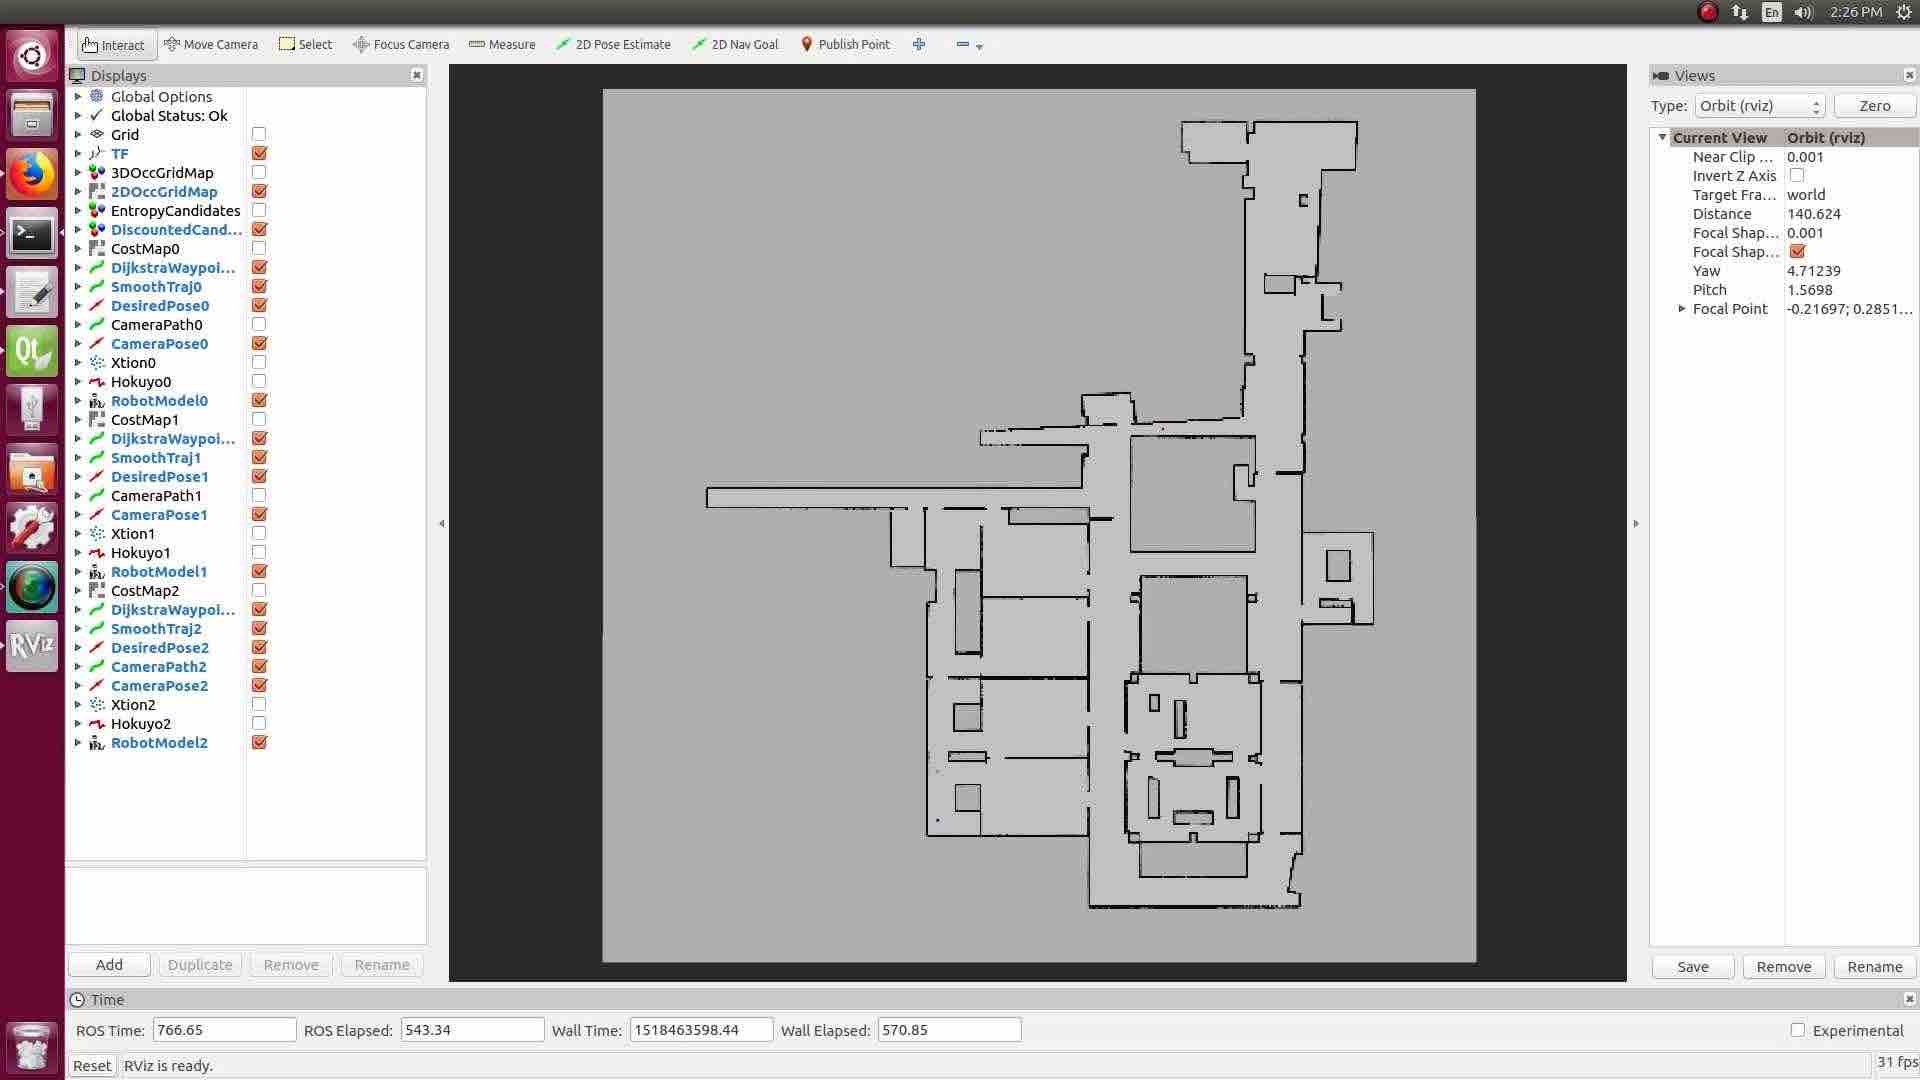
\includegraphics[trim={22cm 5cm 16cm 3.5cm}, clip, height=0.45\columnwidth]{multi_discount_raw_2D_9min_ss.jpg}}
		}
		\vspace*{0.025\columnwidth}
		\caption{2D Projected Occupancy Grid Map of SEH Second Floor}
			\label{fig:sim2Dmaps}
	\end{figure}
	
	
The resulting 3D occupancy grid shows a nearly-completed map after three quadrotors cooperatively explored over $10$ minutes, which is quantified with total map entropy from \refeqn{ShannonsEntropyMap}, shown in Fig. \ref{fig:simH}. An important observation is that the majority of map space was unreachable by any robot, so about $1.2\times10^7$ of the entropy metric could not be improved, regardless of mapping or exploration strategy.

Special attention had to be placed on parameter selection for the bump function and collision-avoidance. For the bump function, increasing the parameter $\beta$ narrows the bump, placing a stronger influence on nearby candidates. However, this choice corresponds to the bump function decreasing at a negligible rate beyond a close neighborhood of the robot, i.e., a large range of distances yield $\mathcal B\approx\mathcal B_\text{far}$. Hence, there is a tradeoff between prioritization of local movements and being able to differentiate the effects of distance on large trajectories.

When robots competed for future poses in a centralized auction framework, the repeated optimizations provided an effective multi-vehicle exploration policy. Between auctions, only a small set of candidates within the neighborhood of the last auction-winning candidate require consideration when updating expected information gains with \refeqn{ExpectedMeasRay} and avoiding collisions between robots using \refeqn{CollisionAvoidanceAmongRobots}, both of which modify the optimization of \refeqn{OptPoseMulti}. Since bidding is applied efficiently, its computation time is negligible compared with other parts of the exploration update such as computing the initial candidate information gains and robot cost maps.

% discounting function \refeqn{discount} has an important parameter, namely $\rho_\text{max}$, which determines the size of the circular region around the robot where discounts are applied. Once again, the parameter introduces a tradeoff; small values of $\rho_\text{discount}$ increase the probability of coverage overlaps and collisions, but larger values only promote a single vehicle from viewing a particular uncertain space. The authors found that lower values of $\rho_\text{max}$ (in this case $3$m was chosen) performed better because the receding horizon updating framework in conjunction with bidding discounting quickly exposes coverage overlaps or possible future collisions. Furthermore, a small $\rho_\text{max}$ has less impact on \refeqn{CandidateBidMulti}, and thus the exploration algorithm is closer to optimal.

% discussion on bump function and discount

	\begin{figure}
		\centerline{
			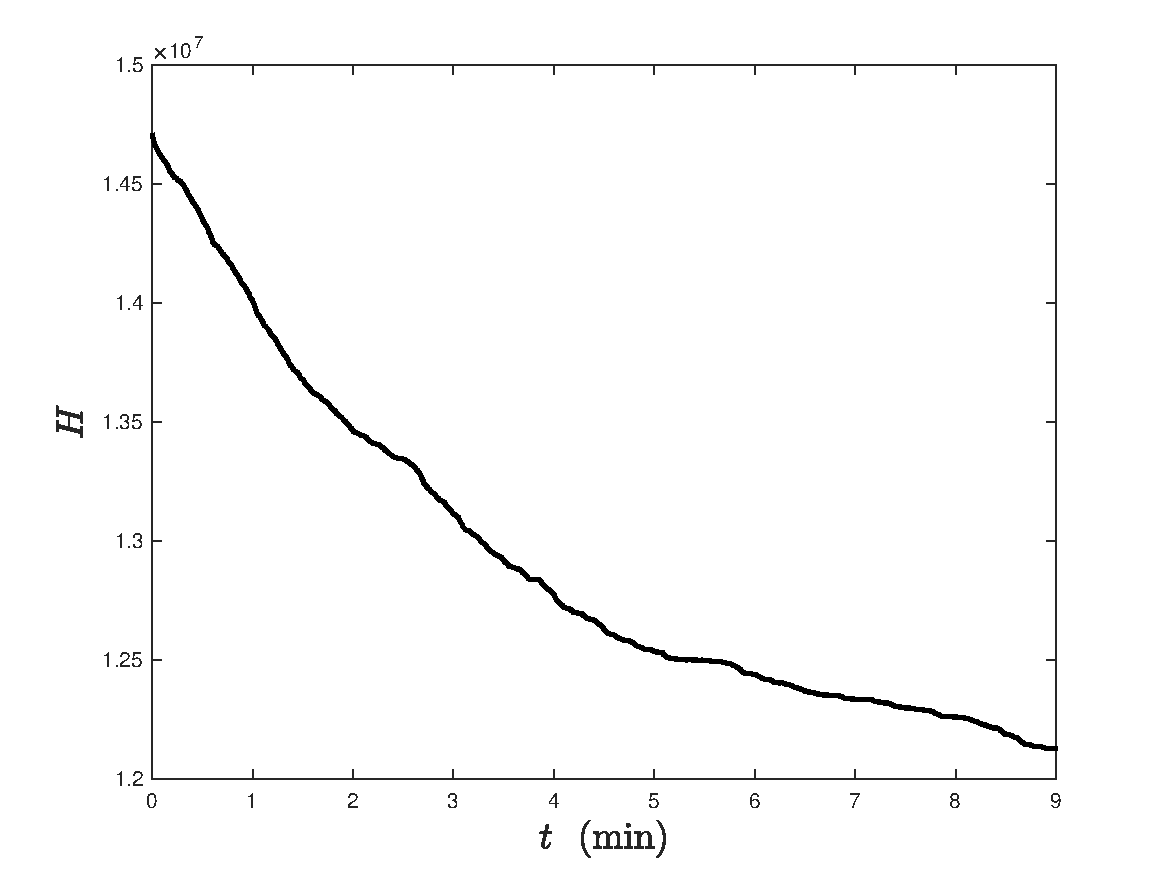
\includegraphics[width=0.9\columnwidth]{multi_H.pdf}
		}
		\caption{Total 3D Map Cell Entropy}
		\label{fig:simH}
	\end{figure}
	
\section{Conclusions}
\label{sec:Conclusions}

This paper introduced a bidding-based solution to the multi-vehicle exploration problem using repeated optimizations of expected map entropy changes and travel distances. The proposed approach integrates recent developments in obtaining occupancy grid probabilities and entropies into several auctions to assign tasks to robots. The bidding process relies on expected map information gains and travel distances, and modifies bids between auctions to promote robotic cooperation. Information gains are modified by updating a temporary expected map. Then, an additional term prevents collisions among robots. Furthermore, a receding horizon constantly updates the bidding process and improves collision avoidance within a dynamic environment. The efficacy of the approach is shown with a numerical simulation, with several computational enhancements for scalability of the algorithms.% Future work includes capturing more features with a 3D exploration map and employing a distributed framework for mapping and exploration.


\bibliography{../../BibSources}% master source for all publications always 2 directories up
\bibliographystyle{IEEEtran}

\end{document}
